%
% EE-457 Design Project #3: 3-GHz Coaxial-Fed Microstrip Patch Antenna
% WNE College of Engineering - Beamer Presentation
% Steven Placzek - November 2025
%

%%%%%%%%%%%%%%%%%%%%%%%%%%%%%%% beamer %%%%%%%%%%%%%%%%%%%%%%%%%%%%%%%%%%%%%%%%%
\documentclass[compress,aspectratio=169,10pt]{beamer}

% Set paper size explicitly to 11.5 x 8 inches in landscape


% Beamer is naturally landscape; the geometry settings above
% ensure the physical page size is 11.5 x 8 in and content fills it.
\mode<presentation>
\raggedbottom % allow variable frame heights to avoid underfull vbox warnings

\usetheme{Warsaw}
\useoutertheme[subsection=true]{smoothbars}

%%%%%%%%%%%%%%%%%%%%%%%%%%%%%%%%%%%%%%%%%%%%%%%%%%%%%%%%%%%%%%%%%%%%%%%%%%%%%%%%%%
% FONTS - Times New Roman style using TeX Gyre Termes (XeLaTeX)
%%%%%%%%%%%%%%%%%%%%%%%%%%%%%%%%%%%%%%%%%%%%%%%%%%%%%%%%%%%%%%%%%%%%%%%%%%%%%%%%%%
\usepackage{fontspec}
\setmainfont{TeX Gyre Termes}
\setsansfont{TeX Gyre Termes}
\setmonofont{DejaVu Sans Mono}

% Empty footer (page numbers added separately)
\setbeamertemplate{footline}[text line]{}

%%%%%%%%%%%%%%%%%%%%%%%%%%%%%%%%%%%%%%%%%%%%%%%%%%%%%%%%%%%%%%%%%%%%%%%%%%%%%%%%%%
% WNE BRAND COLORS
%%%%%%%%%%%%%%%%%%%%%%%%%%%%%%%%%%%%%%%%%%%%%%%%%%%%%%%%%%%%%%%%%%%%%%%%%%%%%%%%%%
\definecolor{WNEBlue}{HTML}{002D72}
\definecolor{WNEGold}{HTML}{F2A900}
\definecolor{WNELightBlue}{HTML}{E6EBF4}
\definecolor{WNEDarkGold}{HTML}{FFFFFF}
\definecolor{WNEGray}{HTML}{FFFFFF}
\definecolor{WNELightGray}{HTML}{FFFFFF}

% Additional utility colors
\definecolor{Red}{rgb}{1,0,0}
\definecolor{Blue}{rgb}{0,0,1}
\definecolor{Green}{rgb}{0,1,0}
\definecolor{darkgreen}{rgb}{0,0.5,0}
\definecolor{darkred}{rgb}{0.75,0,0}

% Layout helper length (gap between logo and horizontal bars)
\newlength{\WNELogoGap}
\setlength{\WNELogoGap}{2.1cm}

%%%%%%%%%%%%%%%%%%%%%%%%%%%%%%%%%%%%%%%%%%%%%%%%%%%%%%%%%%%%%%%%%%%%%%%%%%%%%%%%%%
% APPLY WNE COLORS TO BEAMER THEME
%%%%%%%%%%%%%%%%%%%%%%%%%%%%%%%%%%%%%%%%%%%%%%%%%%%%%%%%%%%%%%%%%%%%%%%%%%%%%%%%%%

% Structure colors
\setbeamercolor{structure}{fg=WNEBlue}
\setbeamercolor{frametitle}{fg=black,bg=}
\setbeamercolor{framesubtitle}{fg=black}

% Title page
\setbeamercolor{title}{fg=white}
\setbeamercolor{subtitle}{fg=WNEGold}
\setbeamercolor{author}{fg=white}
\setbeamercolor{institute}{fg=WNELightBlue}
\setbeamercolor{date}{fg=WNEGold}
\setbeamercolor{title in head/foot}{fg=white,bg=WNEBlue}

% Navigation bar (smoothbars) - text + inline nav bubble
\setbeamercolor{section in head/foot}{fg=WNEBlue,bg=}
\setbeamercolor{subsection in head/foot}{fg=WNEBlue,bg=}

% Palette colors for Warsaw theme
\setbeamercolor{palette primary}{fg=white,bg=WNEBlue}
\setbeamercolor{palette secondary}{fg=white,bg=WNEBlue!85}
\setbeamercolor{palette tertiary}{fg=white,bg=WNEBlue!70}
\setbeamercolor{palette quaternary}{fg=WNEBlue,bg=WNEGold}

% Sidebar
\setbeamercolor{sidebar}{bg=WNEBlue!10}
\setbeamercolor{sidebar}{parent=palette primary}

% Blocks
\setbeamercolor{block title}{fg=white,bg=WNEBlue}
\setbeamercolor{block body}{fg=black,bg=WNELightBlue}
\setbeamercolor{block title alerted}{fg=WNEBlue,bg=WNEGold}
\setbeamercolor{block body alerted}{fg=black,bg=WNEGold!20}
\setbeamercolor{block title example}{fg=white,bg=WNEGray}
\setbeamercolor{block body example}{fg=black,bg=WNELightGray}

% Items
\setbeamercolor{itemize item}{fg=WNEBlue}
\setbeamercolor{itemize subitem}{fg=WNEGold}
\setbeamercolor{itemize subsubitem}{fg=WNEGray}
\setbeamercolor{enumerate item}{fg=WNEBlue}
\setbeamercolor{enumerate subitem}{fg=WNEGold}

% Bullets
\setbeamertemplate{itemize item}[circle]
\setbeamertemplate{itemize subitem}[square]
\setbeamertemplate{itemize subsubitem}[triangle]

% Table of contents
\setbeamercolor{section in toc}{fg=WNEBlue}
\setbeamercolor{subsection in toc}{fg=WNEGray}
\setbeamertemplate{section in toc}[circle]
\setbeamertemplate{subsection in toc}[square]

% Hyperlinks
\hypersetup{
    colorlinks=true,
    linkcolor=WNEBlue,
    urlcolor=WNEBlue,
    citecolor=WNEGold
}

% Navigation symbols
\setbeamertemplate{navigation symbols}{}

%%%%%%%%%%%%%%%%%%%%%%%%%%%%%%%%%%%%%%%%%%%%%%%%%%%%%%%%%%%%%%%%%%%%%%%%%%%%%%%%%%
% FONT SIZE ADJUSTMENTS - slightly smaller global fonts
%%%%%%%%%%%%%%%%%%%%%%%%%%%%%%%%%%%%%%%%%%%%%%%%%%%%%%%%%%%%%%%%%%%%%%%%%%%%%%%%%%
\setbeamerfont{normal text}{size=\small}
\setbeamerfont{frametitle}{size=\normalsize}
\setbeamerfont{framesubtitle}{size=\small}
\setbeamerfont{title}{size=\Large}
\setbeamerfont{subtitle}{size=\normalsize}
\setbeamerfont{author}{size=\normalsize}
\setbeamerfont{institute}{size=\small}
\setbeamerfont{date}{size=\small}
\setbeamerfont{caption}{size=\footnotesize}
\setbeamerfont{section in head/foot}{size=\scriptsize}
\setbeamerfont{subsection in head/foot}{size=\scriptsize}
\AtBeginDocument{\usebeamerfont{normal text}}

% Add frame numbers
\addtobeamertemplate{navigation symbols}{}{%
    \usebeamerfont{footline}%
    \usebeamercolor[fg]{footline}%
    \hspace{1em}%
    \raisebox{1.5pt}[0pt][0pt]{\insertframenumber/\inserttotalframenumber}%
    \hspace{0.5em}%
}

% Mini frame (navigation dot) styling
\setbeamertemplate{mini frames}[box]
\setbeamersize{mini frame size=0.8ex, mini frame offset=0.5ex}
\setbeamercolor{mini frame}{fg=black,bg=black}
\setbeamercolor{mini frame in current section}{fg=black,bg=black}
\setbeamercolor{mini frame in current subsection}{fg=black,bg=black}

% Section and subsection navigation appearance: text with adjacent bubble
\setbeamercolor{section in head/foot}{fg=WNEBlue,bg=}
\setbeamercolor{section in head/foot shaded}{fg=black!45,bg=}
\setbeamercolor{subsection in head/foot}{fg=WNEBlue,bg=}
\setbeamercolor{subsection in head/foot shaded}{fg=black!45,bg=}
\setbeamertemplate{section in head/foot}{%
    \hbox{%
        \insertsectionhead%
        \hspace{0.3ex}%
        {\color{WNEBlue}\raisebox{0.25ex}{\tiny$\bullet$}}%
        \hspace{1.6ex}%
    }%
}
\setbeamertemplate{section in head/foot shaded}{%
    \hbox{%
        \insertsectionhead%
        \hspace{0.3ex}%
        {\color{black!45}\raisebox{0.25ex}{\tiny$\circ$}}%
        \hspace{1.6ex}%
    }%
}
\setbeamertemplate{subsection in head/foot}{%
    \hbox{%
        \insertsubsectionhead%
        \hspace{0.3ex}%
        {\color{WNEBlue}\raisebox{0.2ex}{\tiny$\bullet$}}%
        \hspace{1.4ex}%
    }%
}
\setbeamertemplate{subsection in head/foot shaded}{%
    \hbox{%
        \insertsubsectionhead%
        \hspace{0.3ex}%
        {\color{black!45}\raisebox{0.2ex}{\tiny$\circ$}}%
        \hspace{1.4ex}%
    }%
}

% Custom headline helper: section text + dots on one row
\newcommand{\WNEContentHeadline}{%
    % Small offset from very top margin + requested gap
    \vspace*{0.25cm}%
    \vskip0.4ex%
    % Top navigation row: sections with inline bubbles (short titles)
    \begin{beamercolorbox}[wd=\paperwidth,ht=2.5ex,dp=1ex]{section in head/foot}%
        \usebeamerfont{section in head/foot}%
        \hbox to \paperwidth{%
            \hfill
            {\color{WNEBlue}\insertsectionnavigationhorizontal{0.9\paperwidth}{\hskip1em}{}}%
            \hfill
        }%
    \end{beamercolorbox}%
    % Second navigation row: subsections with inline bubbles (short titles)
    \begin{beamercolorbox}[wd=\paperwidth,ht=2.3ex,dp=1ex]{subsection in head/foot}%
        \usebeamerfont{subsection in head/foot}%
        \hbox to \paperwidth{%
            \hfill
            {\color{WNEBlue}\insertsubsectionnavigationhorizontal{0.9\paperwidth}{\hskip0.75em}{}}%
            \hfill
        }%
    \end{beamercolorbox}%
    % Stripes and info bar
    \begin{beamercolorbox}[wd=\paperwidth,ht=1.3cm,dp=0pt]{section in head/foot}%
        \begin{tikzpicture}[overlay]
            % Top double stripe (full width)
            \fill[WNEBlue] (0,1.15cm) rectangle (\paperwidth,1.20cm);
            \fill[WNEBlue] (0,1.05cm) rectangle (\paperwidth,1.10cm);
            % Bottom double stripe (full width)
            \fill[WNEBlue] (0,0.15cm) rectangle (\paperwidth,0.20cm);
            \fill[WNEBlue] (0,0.05cm) rectangle (\paperwidth,0.10cm);
            % Course info on left
            \node[anchor=west,inner sep=0pt,font=\scriptsize] at (0.05cm,0.62cm) {%
                \begin{tabular}{c}
                    EE-457\\
                    Wave Tx and Rx\\
                    Design Project 03
                \end{tabular}%
            };
            % Current subsection (or section if no subsection) centered between stripes (short titles)
            \node[anchor=center,inner sep=0pt,font=\small\bfseries] at (0.5\paperwidth,0.62cm) {%
                \ifx\insertsubsection\relax
                    \insertsectionhead
                \else
                    \insertsubsectionhead
                \fi
            };
            % WNE Logo on right side
            \node[anchor=east,inner sep=0pt] at (\paperwidth-0.35cm,0.62cm) {%
                
\includegraphics[height=0.8cm]{img/wne-icon-trimmed.png}%
            };
        \end{tikzpicture}%
    \end{beamercolorbox}%
}

% Default headline for content slides
\setbeamertemplate{headline}{\WNEContentHeadline}
% Suppress automatic section/subsection title pages from the theme
\setbeamertemplate{section page}{}
\setbeamertemplate{subsection page}{}

% Replace theme-provided section intro frames with a compact outline slide
% No automatic section/subsection splash frames
\AtBeginSection[]{}
\AtBeginSubsection[]{}

% Add extra space between headline and frametitle bar
\addtobeamertemplate{headline}{}{\vskip12pt}

%%%%%%%%%%%%%%%%%%%%%%%%%%%%%%%%%%%%%%%%%%%%%%%%%%%%%%%%%%%%%%%%%%%%%%%%%%%%%%%%%%
% PACKAGES
%%%%%%%%%%%%%%%%%%%%%%%%%%%%%%%%%%%%%%%%%%%%%%%%%%%%%%%%%%%%%%%%%%%%%%%%%%%%%%%%%%
\usepackage{subfigure}
\usepackage{multicol}
\usepackage{amsmath}
\usepackage{amssymb}
\usepackage{bm}
\usepackage{graphicx}
\usepackage{booktabs}
\usepackage{siunitx}
\usepackage{tikz}
\usepackage{pdfpages}
\usepackage{hyperref}

% Encoding
\usepackage[english]{babel}

% TikZ libraries
\usetikzlibrary{calc,positioning,shapes.geometric,arrows.meta}

% For background images
\usepackage{eso-pic}

% Code listings for MATLAB
\usepackage{listings}
\usepackage[verbatim]{lstfiracode}
\lstset{
    language=Matlab,
    style=FiraCodeStyle,
    basicstyle=\tiny\ttfamily,
    keywordstyle=\bfseries,
    commentstyle=\color{darkgreen},
    numbers=left,
    numberstyle=\tiny,
    stepnumber=1,
    numbersep=8pt,
    frame=single,
    breaklines=true,
    breakatwhitespace=true,
    showstringspaces=false
}

%%%%%%%%%%%%%%%%%%%%%%%%%%%%%%%%%%%%%%%%%%%%%%%%%%%%%%%%%%%%%%%%%%%%%%%%%%%%%%%%%%
% FIGURE AND TABLE NUMBERING
%%%%%%%%%%%%%%%%%%%%%%%%%%%%%%%%%%%%%%%%%%%%%%%%%%%%%%%%%%%%%%%%%%%%%%%%%%%%%%%%%%
\setbeamertemplate{caption}[numbered]

%%%%%%%%%%%%%%%%%%%%%%%%%%%%%%%%%%%%%%%%%%%%%%%%%%%%%%%%%%%%%%%%%%%%%%%%%%%%%%%%%%
% CUSTOM COMMANDS
%%%%%%%%%%%%%%%%%%%%%%%%%%%%%%%%%%%%%%%%%%%%%%%%%%%%%%%%%%%%%%%%%%%%%%%%%%%%%%%%%%
\newcommand{\emphgold}[1]{\textcolor{WNEGold}{\textbf{#1}}}
\newcommand{\emphblue}[1]{\textcolor{WNEBlue}{\textbf{#1}}}

%%%%%%%%%%%%%%%%%%%%%%%%%%%%%%%%%%%%%%%%%%%%%%%%%%%%%%%%%%%%%%%%%%%%%%%%%%%%%%%%%%
% TITLE PAGE INFO
%%%%%%%%%%%%%%%%%%%%%%%%%%%%%%%%%%%%%%%%%%%%%%%%%%%%%%%%%%%%%%%%%%%%%%%%%%%%%%%%%%

% CoE Logo in corner
\logo{
\includegraphics[height=0.6cm]{img/wne-logo-coe-rev.png}}

\title{Design Project \#03}
\subtitle{3-GHz Coaxial-Fed Microstrip Patch Antenna}
\author{Steven Placzek}
\institute{%
    Western New England University\\
    College of Engineering\\
    Department of Electrical and Computer Engineering
}
\date{EE-457 Wave Transmission and Reception\\Fall 2025}
%%%%%%%%%%%%%%%%%%%%%%%%%%%%%%%%%%%%%%%%%%%%%%%%%%%%%%%%%%%%%%%%%%%%%%%%%%%%%%%%%%
% BEGIN DOCUMENT
%%%%%%%%%%%%%%%%%%%%%%%%%%%%%%%%%%%%%%%%%%%%%%%%%%%%%%%%%%%%%%%%%%%%%%%%%%%%%%%%%%

\begin{document}
\includepdf[pages={1-2}]{EE_457_Design_Project_03_-_Original_File.pdf}
%%%%%%%%%%%%%%%%%%%%%%%%%%%%%%%%%%%%%%%%%%%%%%%%%%%%%%%%%%%%%%%%%%%%%%%%%%%%%%%%%%
% TITLE SLIDE WITH CUSTOM LAYOUT
%%%%%%%%%%%%%%%%%%%%%%%%%%%%%%%%%%%%%%%%%%%%%%%%%%%%%%%%%%%%%%%%%%%%%%%%%%%%%%%%%%
{
\setbeamertemplate{headline}{%
    % Stripes only for title page (no navigation)
    \begin{beamercolorbox}[wd=\paperwidth,ht=1.3cm,dp=0pt]{section in head/foot}%
        \begin{tikzpicture}[overlay]
            % Top double stripe (lowered to center logo between lines)
            \fill[WNEBlue] (0,0.95cm) rectangle (\paperwidth,1.00cm);
            \fill[WNEBlue] (0,0.87cm) rectangle (\paperwidth,0.92cm);
            % Bottom double stripe
            \fill[WNEBlue] (0,0.07cm) rectangle (\paperwidth,0.12cm);
            \fill[WNEBlue] (0,0cm) rectangle (\paperwidth,0.05cm);
            % Author on left
            \node[anchor=west,inner sep=0pt,font=\normalsize\bfseries] at (0.5cm,0.55cm) {%
                Steven Placzek%
            };
            % University info centered
            \node[anchor=center,inner sep=0pt,font=\small] at (0.5\paperwidth,0.55cm) {%
                \begin{tabular}{c}
                    \textbf{Western New England University}\\
                    College of Engineering\\
                    EE-457 Wave Transmission and Reception
                \end{tabular}%
            };
            % WNE Logo on right side
            \node[anchor=east,inner sep=0pt] at (\paperwidth-0.3cm,0.55cm) {%
                
\includegraphics[height=0.9cm]{img/wne-icon-trimmed.png}%
            };
        \end{tikzpicture}%
    \end{beamercolorbox}%
}
\begin{frame}[plain]
    \vspace{1.4cm}
    \begin{center}
        {\Huge\bfseries Design Project \#3}

        \vspace{1em}
        {\Large 3-GHz Coaxial-Fed Microstrip Patch Antenna}

        \vspace{1.5em}
        {\large Steven Placzek}\\[0.25em]
        {\large EE-457 Wave Transmission and Reception}\\[0.15em]
        {\large Western New England University}
    \end{center}

    \vfill
    \begin{flushright}
        
\includegraphics[height=1.3cm]{img/wne-logo-coe.png}
    \end{flushright}
\end{frame}
}

%%%%%%%%%%%%%%%%%%%%%%%%%%%%%%%%%%%%%%%%%%%%%%%%%%%%%%%%%%%%%%%%%%%%%%%%%%%%%%%%%%
% TABLE OF CONTENTS - with section text navigation
%%%%%%%%%%%%%%%%%%%%%%%%%%%%%%%%%%%%%%%%%%%%%%%%%%%%%%%%%%%%%%%%%%%%%%%%%%%%%%%%%%
{
\setbeamertemplate{headline}{%
    \WNEContentHeadline
}
\begin{frame}{Table of Contents}
    \footnotesize
    \begin{columns}[T,onlytextwidth]
        \begin{column}{0.32\textwidth}
            \tableofcontents[sectionstyle=show/show,subsectionstyle=show/show,sections={1-2}]
        \end{column}
        \begin{column}{0.32\textwidth}
            \tableofcontents[sectionstyle=show/show,subsectionstyle=show/show,sections={3-5}]
        \end{column}
        \begin{column}{0.32\textwidth}
            \tableofcontents[sectionstyle=show/show,subsectionstyle=show/show,sections={6-10}]
        \end{column}
    \end{columns}
\end{frame}
}

%%%%%%%%%%%%%%%%%%%%%%%%%%%%%%%%%%%%%%%%%%%%%%%%%%%%%%%%%%%%%%%%%%%%%%%%%%%%%%%%%%
% INTRODUCTION
%%%%%%%%%%%%%%%%%%%%%%%%%%%%%%%%%%%%%%%%%%%%%%%%%%%%%%%%%%%%%%%%%%%%%%%%%%%%%%%%%%

\section[Overview]{Project Overview}

\subsection[Objectives \& Specs]{Project Objectives, Specifications, Initial Parameters, \& HFSS Setup}

% \begin{frame}{Project Objectives and Specifications}
%     \textbf{Design Objectives}
%     \begin{itemize}
%         \item Design a \textbf{3-GHz} coaxial-fed microstrip patch antenna on FR4 ($h = 1.5748$~mm, $\varepsilon_r = 4.4$, $\tan\delta = 0.02$)
%         \item Set patch width target $\text{W} \approx 1.5 \cdot \texttt{L\_e}$
%         \item Meet input return loss at 3~GHz: $|S_{11}| \le -30$~dB
%         \item Characterize gain, directivity, E/H beam-widths, and radiation efficiency
%     \end{itemize}
% \end{frame}

\begin{frame}{Project Overview}
    \begin{columns}[T]
        \begin{column}{0.55\textwidth}
            \textbf{Design Objectives:}
            \begin{itemize}
                \item Design a 3-GHz coaxial-fed microstrip patch antenna
                \item Substrate: 62-mil thick FR4 ($h = 1.5748$~mm)
                \item Dielectric properties: $\varepsilon_r = 4.4$, $\tan\delta = 0.02$
                \item Patch width: $W \approx 1.5 L_e$
            \end{itemize}
            
            \vspace{0.5em}
            \textbf{Target Specifications:}
            \begin{itemize}
                \item Input return loss at 3~GHz: $|S_{11}| \le -30$~dB
                \item Characterize gain, directivity, and Beam-widths
            \end{itemize}
        \end{column}
        \begin{column}{0.42\textwidth}
            \centering
            \vspace*{-0.5cm}
            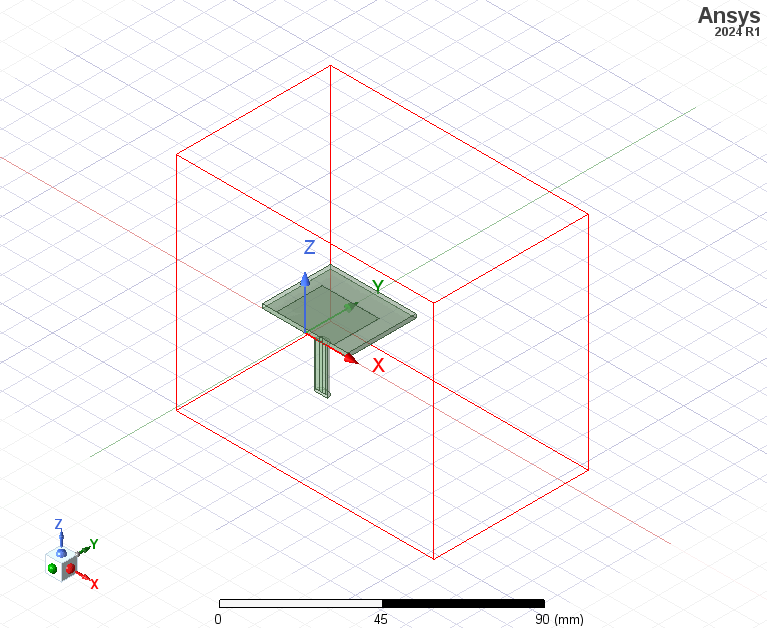
\includegraphics[width=\textwidth]{./img/Model_Layout_3D.png}
            \vspace{0.3em}
            \small\textit{3D HFSS Model}
        \end{column}
    \end{columns}
\end{frame}

%%%%%%%%%%%%%%%%%%%%%%%%%%%%%%%%%%%%%%%%%%%%%%%%%%%%%%%%%%%%%%%%%%%%%%%%%%%%%%%%%%
% Table 1
%%%%%%%%%%%%%%%%%%%%%%%%%%%%%%%%%%%%%%%%%%%%%%%%%%%%%%%%%%%%%%%%%%%%%%%%%%%%%%%%%%
\section[Table 1]{Table 1}

\subsection[Table 1]{Table 1: Microstrip Patch Design Parameters Calculated in Matlab \copyright}

\begin{frame}
    \begin{table}[!ht]
        \centering
        \footnotesize
        \begin{tabular}{|c|c|c|}
            \hline
            \textbf{Parameter} & \textbf{Calculated} & \textbf{Unit} \\
            \hline
            $f_0$ & 3.0000 & GHz \\
            \hline
            $h$ & 1.5748 & mm \\
            \hline
            $\varepsilon_r$ & 4.4 & -- \\
            \hline
            $\lambda_g$ & 47.6401 & mm \\
            \hline
            $L_e$ & 23.8201 & mm \\
            \hline
            $W'$ & 35.7301 & mm \\
            \hline
            $\varepsilon_{r,\text{eff}}$ & 4.4000 & -- \\
            \hline
            $\Delta L$ & 726.7002 & $\mu$m \\
            \hline
            $L_p$ & 22.3667 & mm \\
            \hline
            $W$ & 35.7301 & mm \\
            \hline
            $R_{\text{Edge}}$ & 239.4675 & $\Omega$ \\
            \hline
            $x_f$ & 8.3119 & mm \\
            \hline
        \end{tabular}
        \caption{Calculated design parameters for the 3-GHz coaxial-fed microstrip patch antenna}
        \label{tab:table-1-calculated-params}
    \end{table}
\end{frame}
%%%%%%%%%%%%%%%%%%%%%%%%%%%%%%%%%%%%%%%%%%%%%%%%%%%%%%%%%%%%%%%%%%%%%%%%%%%%%%%%%%
% Table 2 | HFSS OPTIMETRIC SWEEP RESULTS
%%%%%%%%%%%%%%%%%%%%%%%%%%%%%%%%%%%%%%%%%%%%%%%%%%%%%%%%%%%%%%%%%%%%%%%%%%%%%%%%%%
\section[Table 2]{Table 2}

\subsection[Table 2]{Table 2: Geometry Parameters per HFSS Optimetric Sweep}
\begin{frame}
    \begin{table}
        \centering
        \footnotesize
        \begin{tabular}{|c|c|c|c|c|c|}
            \hline
            \textbf{Parameter} & \textbf{V1} & \textbf{V2} & \textbf{V3} & \textbf{V4} & \textbf{Unit} \\
            \hline
            $L_e$ & 23.8201 & 23.8201 & 23.8201 & 24.0187 & mm \\
            \hline
            $\Delta L$ & 726.7001 & 726.7001 & 726.7001 & 726.7001 & $\mu$m \\
            \hline
            $L$ & 22.3667 & 22.3667 & 22.3667 & 22.5652 & mm \\
            \hline
            $W$ & 35.7302 & 35.7302 & 35.7302 & 36.0279 & mm \\
            \hline
            $x_f$ & 8.3119 & 8.3119 & 8.3119 & 5.8183 & mm \\
            \hline
            $x_0$ & 3.5982 & 3.5982 & 3.5982 & 6.1910 & mm \\
            \hline
            $L_s$ & 33.5501 & 33.5501 & 33.5501 & 33.8478 & mm \\
            \hline
            $W_s$ & 53.5952 & 53.5952 & 53.5952 & 54.0418 & mm \\
            \hline
        \end{tabular}
        \caption{\small Simulated parameters for HFSS optimetric sweep of $X_{\text{sweep}}$. Note: V2 and V3 did not see any improvements for $|S_{11}|_{\text{dB}}$ after running another sweep, despite changing the step size to 0.02.}
	        \label{tab:simulated-params}
	    \end{table}
\end{frame}
%%%%%%%%%%%%%%%%%%%%%%%%%%%%%%%%%%%%%%%%%%%%%%%%%%%%%%%%%%%%%%%%%%%%%%%%%%%%%%%%%%
% Table 3 | HFSS ANTENNA PARAMETERS
%%%%%%%%%%%%%%%%%%%%%%%%%%%%%%%%%%%%%%%%%%%%%%%%%%%%%%%%%%%%%%%%%%%%%%%%%%%%%%%%%%
\section[Table 3]{Table 3}

\subsection[Table 3]{Table 3: HFSS Antenna Parameters}

\begin{frame}
    \begin{table}
        \centering
        \begin{tabular}{|l|c|c|}
            \hline
            \textbf{Parameter} & \textbf{HFSS} & \textbf{Unit} \\
            \hline
            $D$ & 5.09 & W/W \\
            \hline
            $D$ & 7.07 & dB \\
            \hline
            $G$ & 2.42 & W/W \\
            \hline
            $G$ & 3.84 & dB \\
            \hline
            $BW_{EP}$ & 102.94 & $^\circ$ \\
            \hline
            $BW_{HP}$ & 78.68 & $^\circ$ \\
            \hline
            $e_{\text{rad}}$ & 47.5 & \% \\
            \hline
        \end{tabular}
        \caption{Simulated directivity, gain, beam-width, and radiation efficiency at 3~GHz}
    \end{table}
\end{frame}

\section[Bandwidth]{\texorpdfstring{$\text{BW}_f$}{BW\_f}}

\subsection[Table 4]{Table 4: 10~dB $\text{BW}_f$ Summary}

\begin{frame}
    \begin{table}
        \centering
        \begin{tabular}{|c|c|c|c|}
            \hline
            \textbf{Parameter} & \textbf{Calculated} & \textbf{HFSS} & \textbf{Unit} \\
            \hline
            $BW_f$ ($-10$~dB) & 21.6673 & 89.7000 & MHz \\
            \hline
            $BW_f$ ($-10$~dB) & 0.7222 & 2.9898 & \% \\
            \hline
        \end{tabular}
        \caption{Calculated and simulated $-10$~dB impedance bandwidth}
        \label{tab:bandwidth-summary}
    \end{table}

    \vspace{1em}
    \begin{block}{Key Finding}
        Achieved approximately \textbf{$3\%$ fractional bandwidth} at the $-10$~dB return loss level for optimized designs (V2--V4).
    \end{block}
\end{frame}

\subsection[Sweeps]{Sweep Bandwidths}

\begin{frame}{Bandwidth Summary by Sweep}
    \begin{table}
        \centering
        \begin{tabular}{|c|c|c|c|c|c|}
            \hline
            \textbf{Parameter} & \textbf{Unit} & \textbf{V1} & \textbf{V2} & \textbf{V3} & \textbf{V4} \\
            \hline
            $BW_f$ ($-10$~dB) & GHz & N/A & 0.0903 & 0.0903 & 0.0897 \\
            \hline
            $BW_f$ ($-10$~dB) & \% & N/A & 2.99 & 2.99 & 2.99 \\
            \hline
        \end{tabular}
        \caption{$-10$~dB bandwidths from $|S_{11}|_\text{(dB)}$ for sweeps V1--V4}
        \label{tab:bandwidth-sweeps}
    \end{table}
\end{frame}

%%%%%%%%%%%%%%%%%%%%%%%%%%%%%%%%%%%%%%%%%%%%%%%%%%%%%%%%%%%%%%%%%%%%%%%%%%%%%%%%%%
% RADIATION PATTERNS
%%%%%%%%%%%%%%%%%%%%%%%%%%%%%%%%%%%%%%%%%%%%%%%%%%%%%%%%%%%%%%%%%%%%%%%%%%%%%%%%%%

\section[Final Design]{Final Microstrip Patch Design: Antenna Parameters}

\subsection[HFSS Params]{Final HFSS Antenna Parameters}

\begin{frame}
    \begin{table}
        \centering
        \small
        \begin{tabular}{|l|c|c|}
            \hline
            \textbf{Quantity} & \textbf{Value} & \textbf{Unit} \\
            \hline
            Frequency $f$ & 3.0000 & GHz \\
            \hline
            Max $U$ & 0.3850 & W/sr \\
            \hline
            Peak directivity & 4.3989 & -- \\
            \hline
            Peak gain & 2.4211 & -- \\
            \hline
            Peak realized gain & 2.4192 & -- \\
            \hline
            Radiated power & 1.0999 & W \\
            \hline
            Accepted power & 1.9984 & W \\
            \hline
            Radiation efficiency & 0.5504 & -- \\
            \hline
            Total efficiency & 0.5500 & -- \\
            \hline
            Front-to-back ratio & 6.1402 & dB \\
            \hline
        \end{tabular}
        \caption{HFSS antenna parameters at $f_0 = 3.0$~GHz for final microstrip patch antenna design.}
        \label{tab:final-antenna-params}
    \end{table}
\end{frame}

\subsection[Gain Plot]{Microstrip Patch Antenna Design Gain (V4)}
\begin{frame}
    \begin{figure}
        \centering
        \vspace*{-0.75cm}
        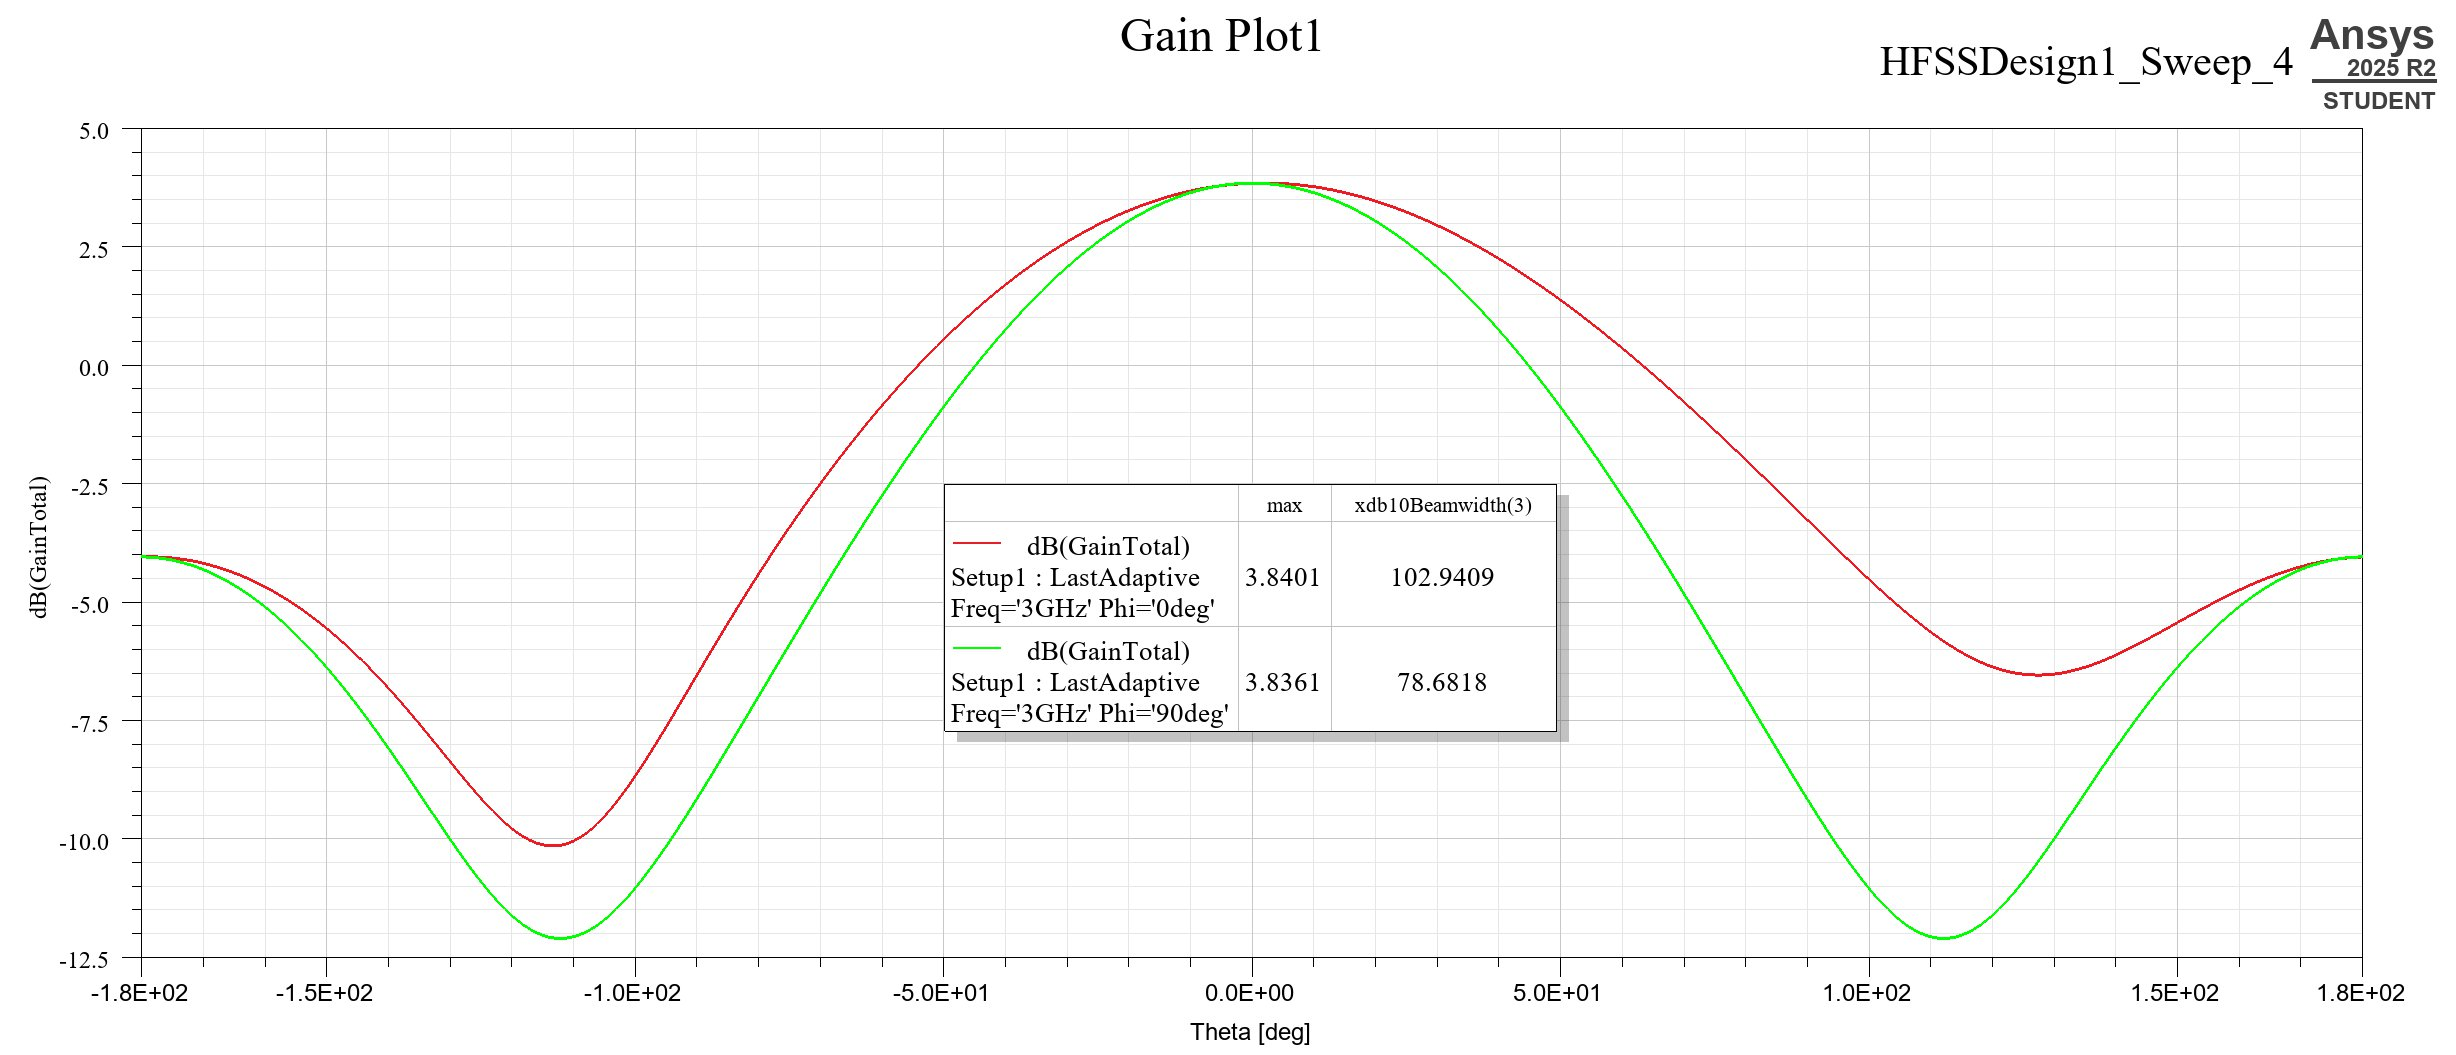
\includegraphics[width=1.05\textwidth,keepaspectratio,clip,trim=0cm 1.25cm 0cm 3.95cm]{img/Gain_Plot_01__Sweep_04.jpg}
        % \caption{Total gain at 3~GHz for the antenna with the final feed position.}
            \caption{Total gain patterns at 3~GHz for the final optimized design, highlighting the 10~dB beam-width in the principal planes.}
    \end{figure}
\end{frame}

% \subsection{10~dB Beam-width}
% \begin{frame}
%     \begin{figure}
%         \centering
%         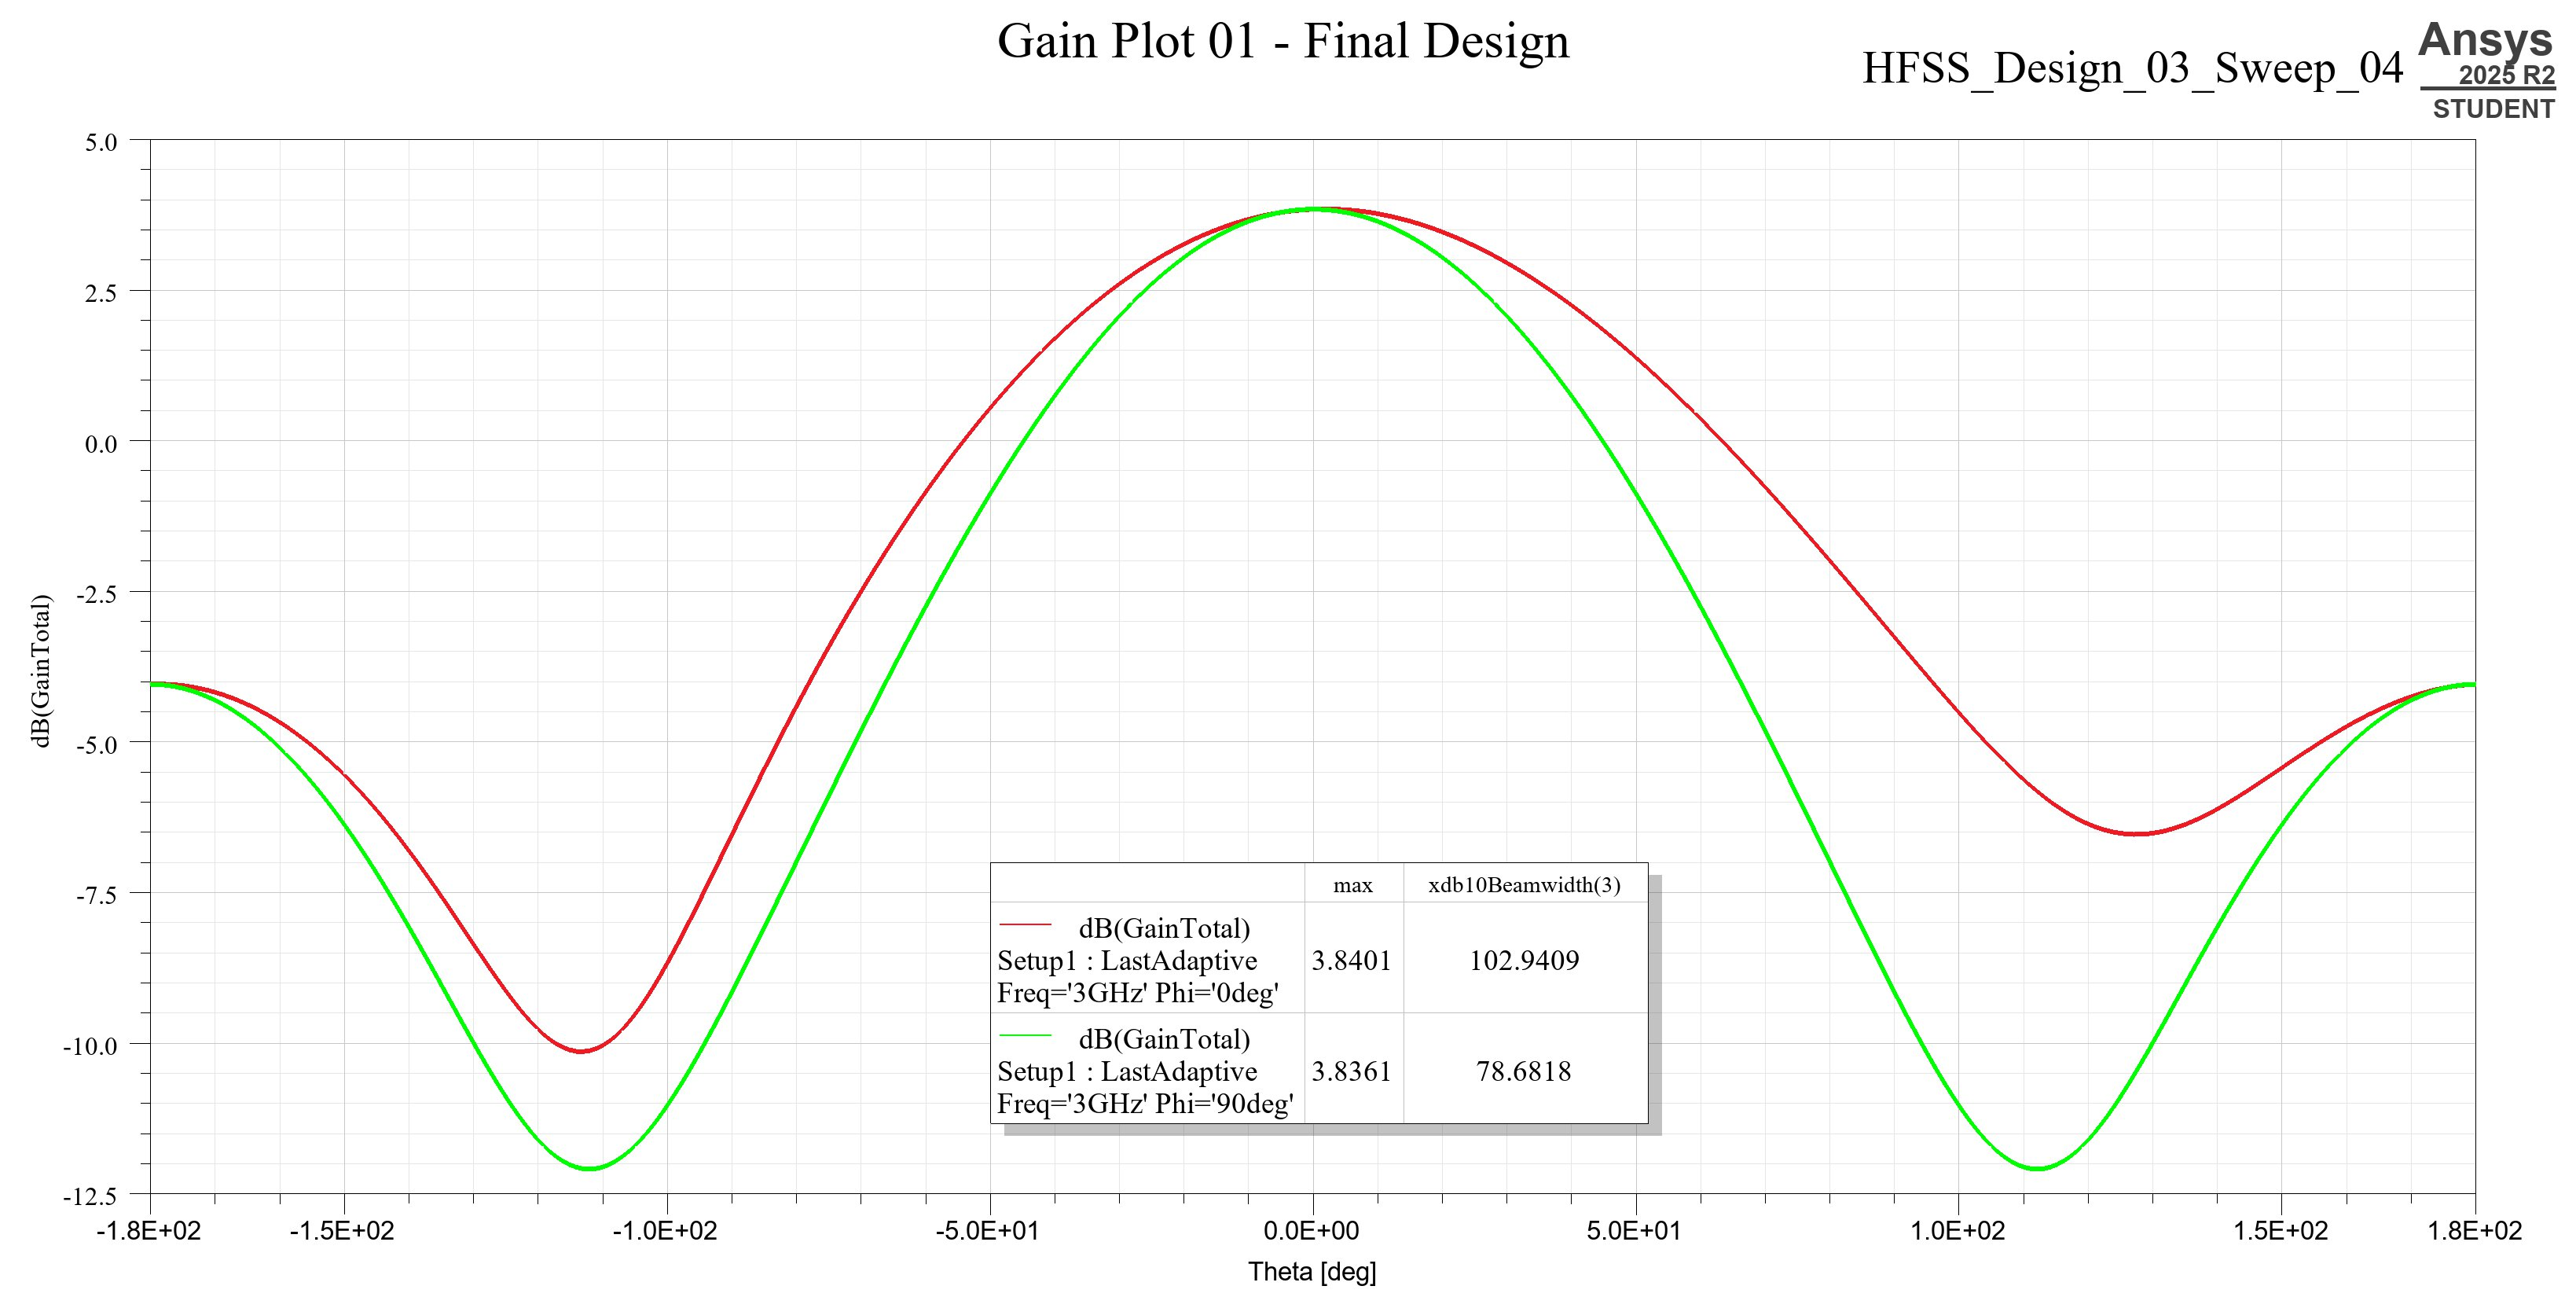
\includegraphics[width=0.95\textwidth,height=0.78\textheight,keepaspectratio,clip,trim=0cm 0.25cm 0cm 0.25cm]{img/Gain_Plot_01__10dB_BeamWidth__Final_Design_Parameters.jpg}
%         \caption{H-Plane \& E-plane 10~dB beam-width}
%     \end{figure}
% \end{frame}

\subsection[Radiation Pattern]{HFSS Simulated Radiation Pattern}
\begin{frame}
    \begin{figure}
        \centering
        \vspace*{-0.5cm}% move figure 2.5cm up from the vertical center
        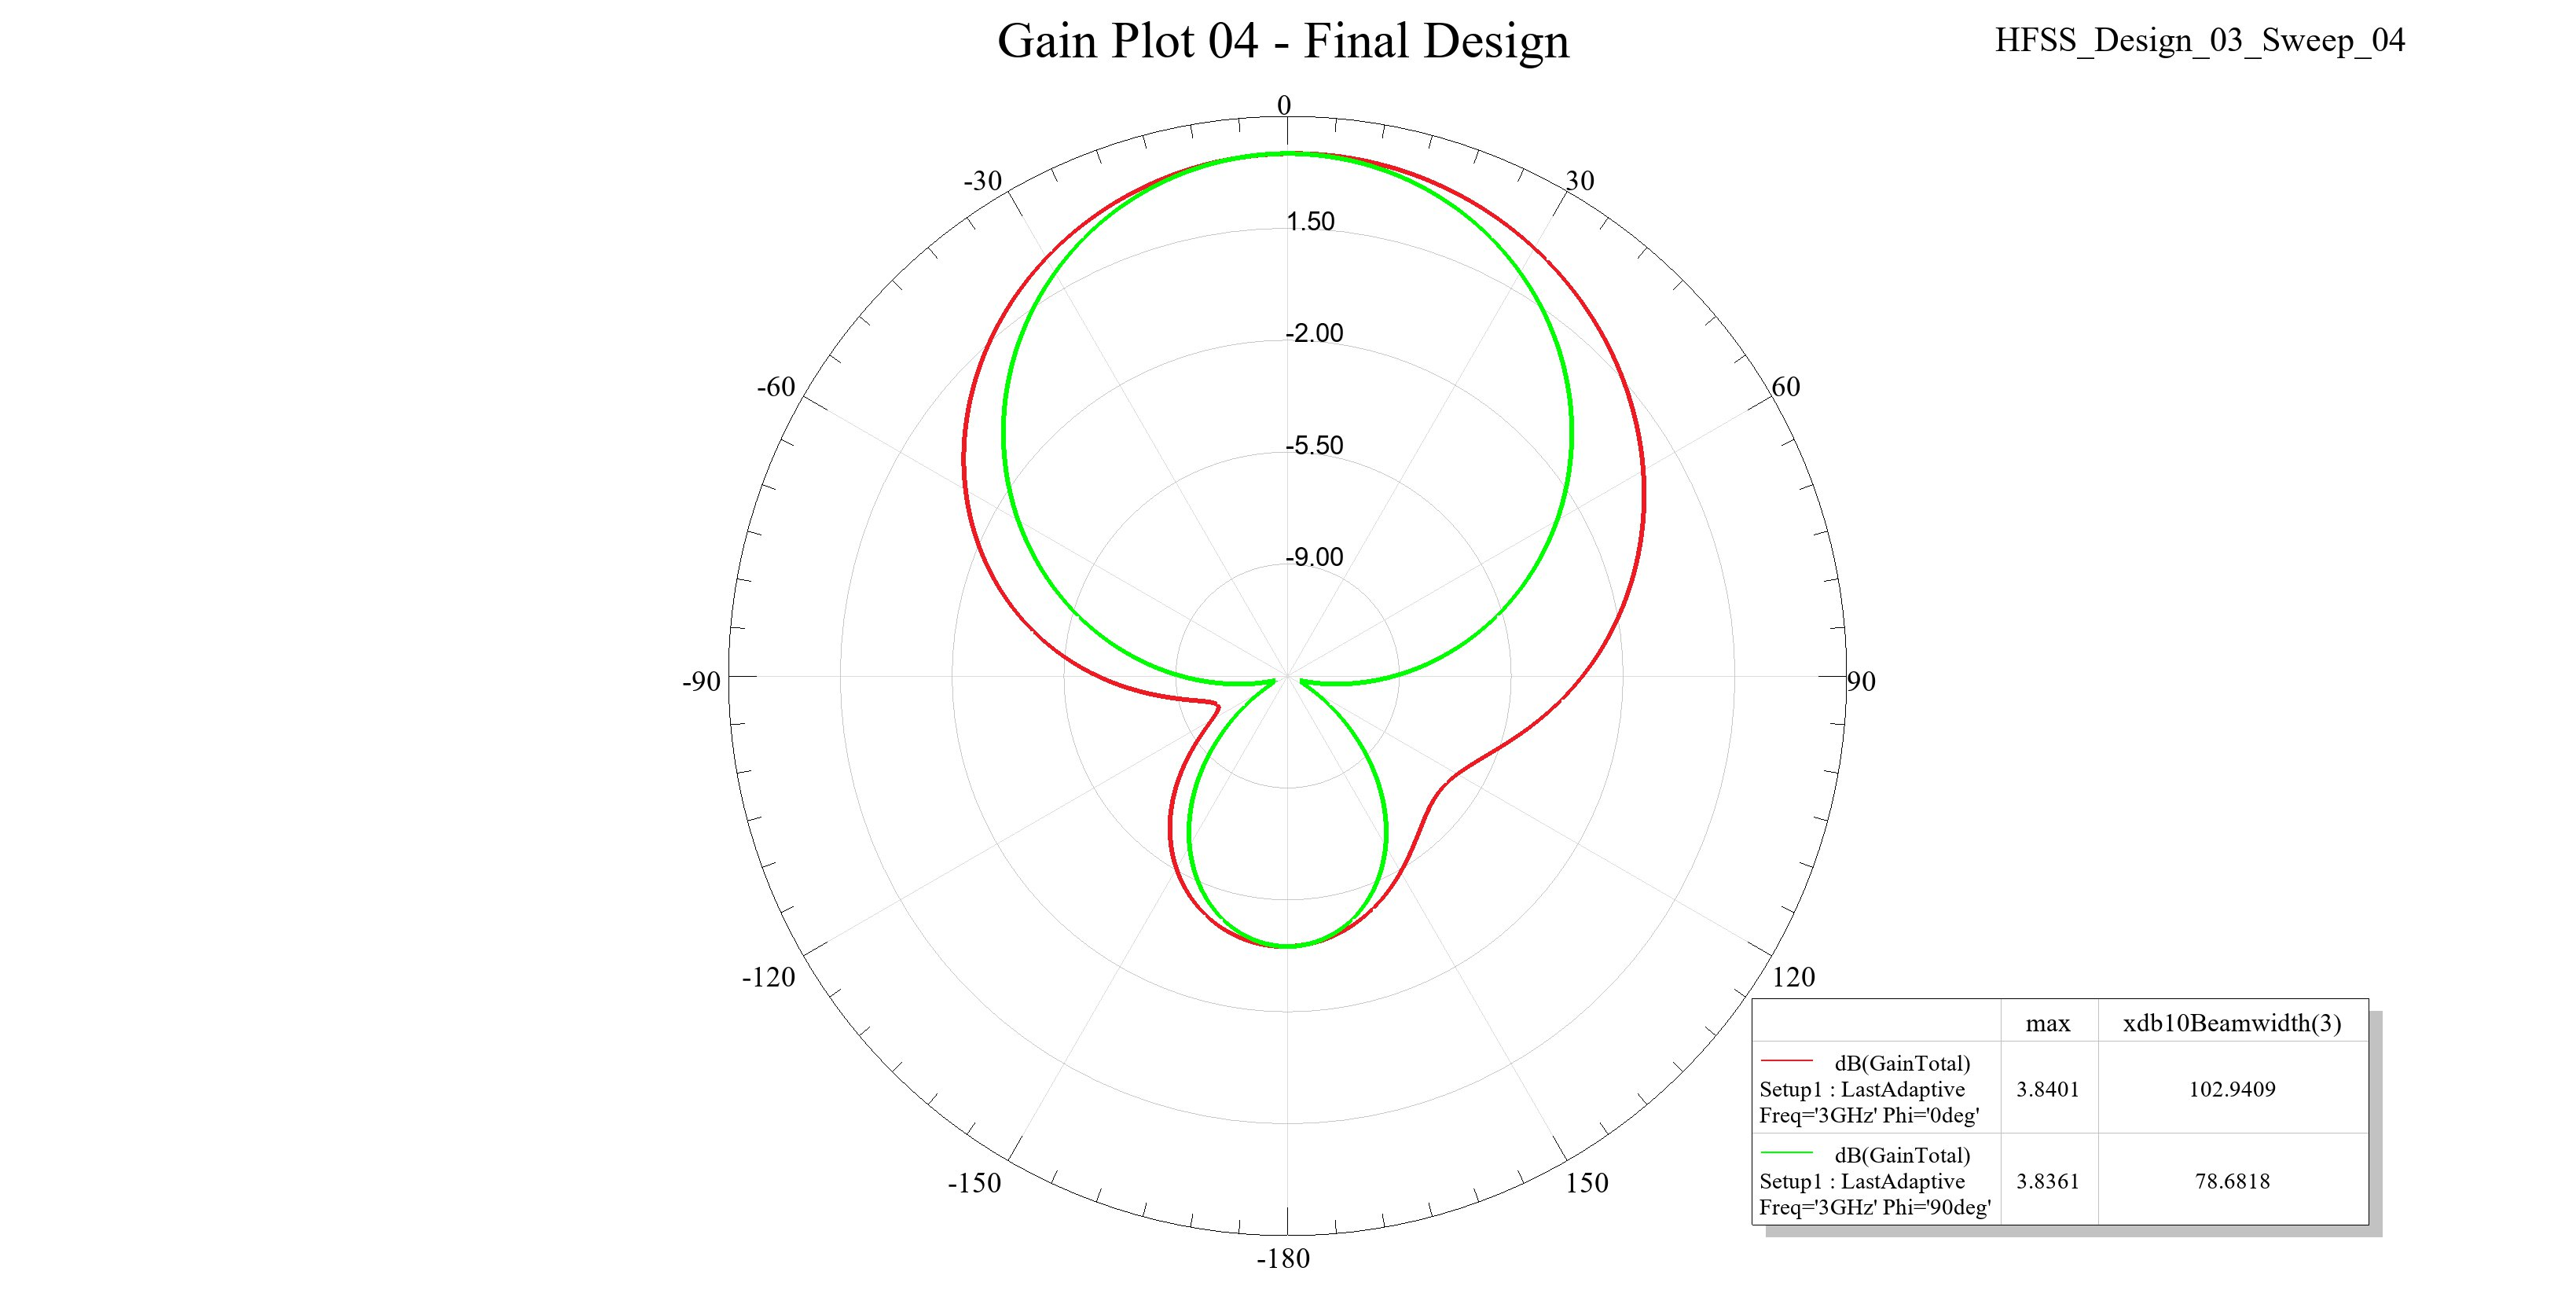
\includegraphics[width=0.85\textwidth,keepaspectratio,clip,trim=0cm 0.25cm 0cm 3.1cm]{img/Gain_Plot_04__10dB_BeamWidth__Final_Design_Parameters.jpg}
        \caption{HFSS Simulated Radiation Pattern with E-plane \& H-plane 10~dB beam-widths.}
        \label{fig:hfss-radiation-pattern}
    \end{figure}
\end{frame}

% \subsection{\texorpdfstring{Microstrip Patch Antenna $|S_{11}|_\text{(dB)}$ {Design S11}}
% \begin{frame}{Microstrip Patch Antenna $|S_{11}|_\text{(dB)}$}
%     \begin{figure}
%         \centering
%         \vspace*{-0.5cm}% move figure 2.5cm up from the vertical center
%         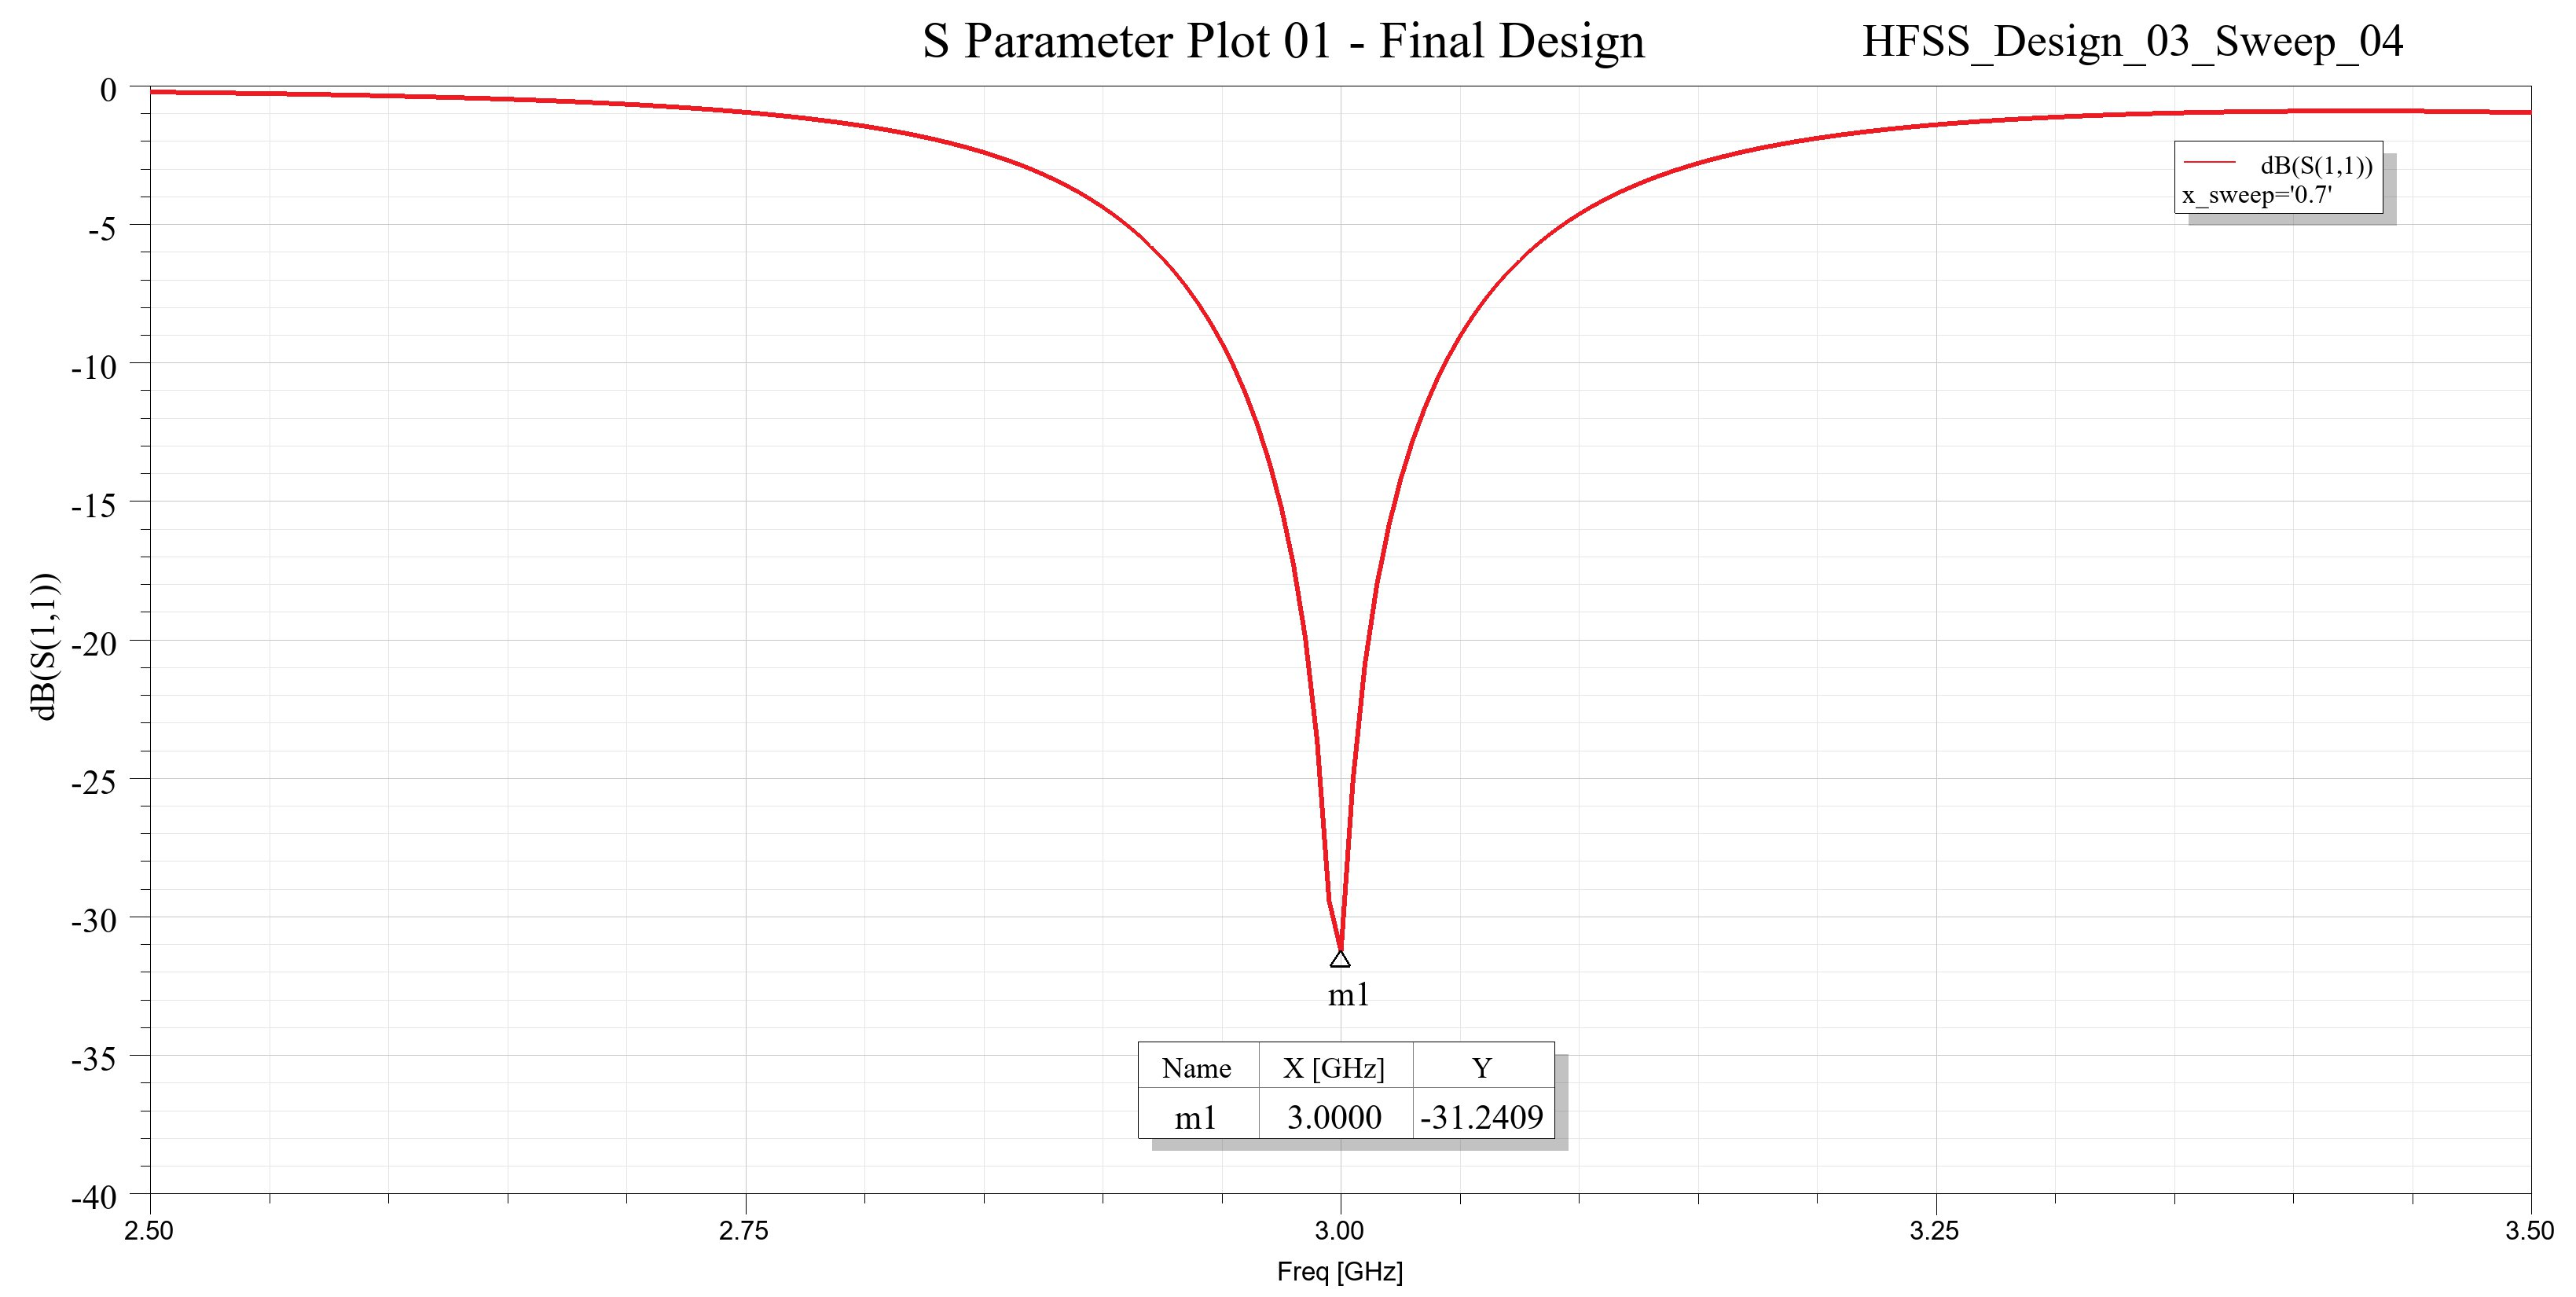
\includegraphics[width=0.95\textwidth,keepaspectratio,clip,trim=0cm 0.25cm 0cm 3.15cm]{img/S_Parameter_Chart_01___Final_Design_S11dB.jpg}
%         \caption{$|S_{11}|_\text{(dB)}$ vs. $f_\text{(GHz)}$ - HFSS sweep from 2.5 GHz to 3.5 GHz.}
%     \end{figure}
% \end{frame}

\subsection[Smith Chart]{\texorpdfstring{Microstrip Patch Antenna Design Impedance Match}{Smith Chart}}

\begin{frame} % {Microstrip Patch Antenna Design: $S_{11}\,\text{(dB)}$}
    \begin{figure}
        \centering
        \vspace*{-0.475cm}
        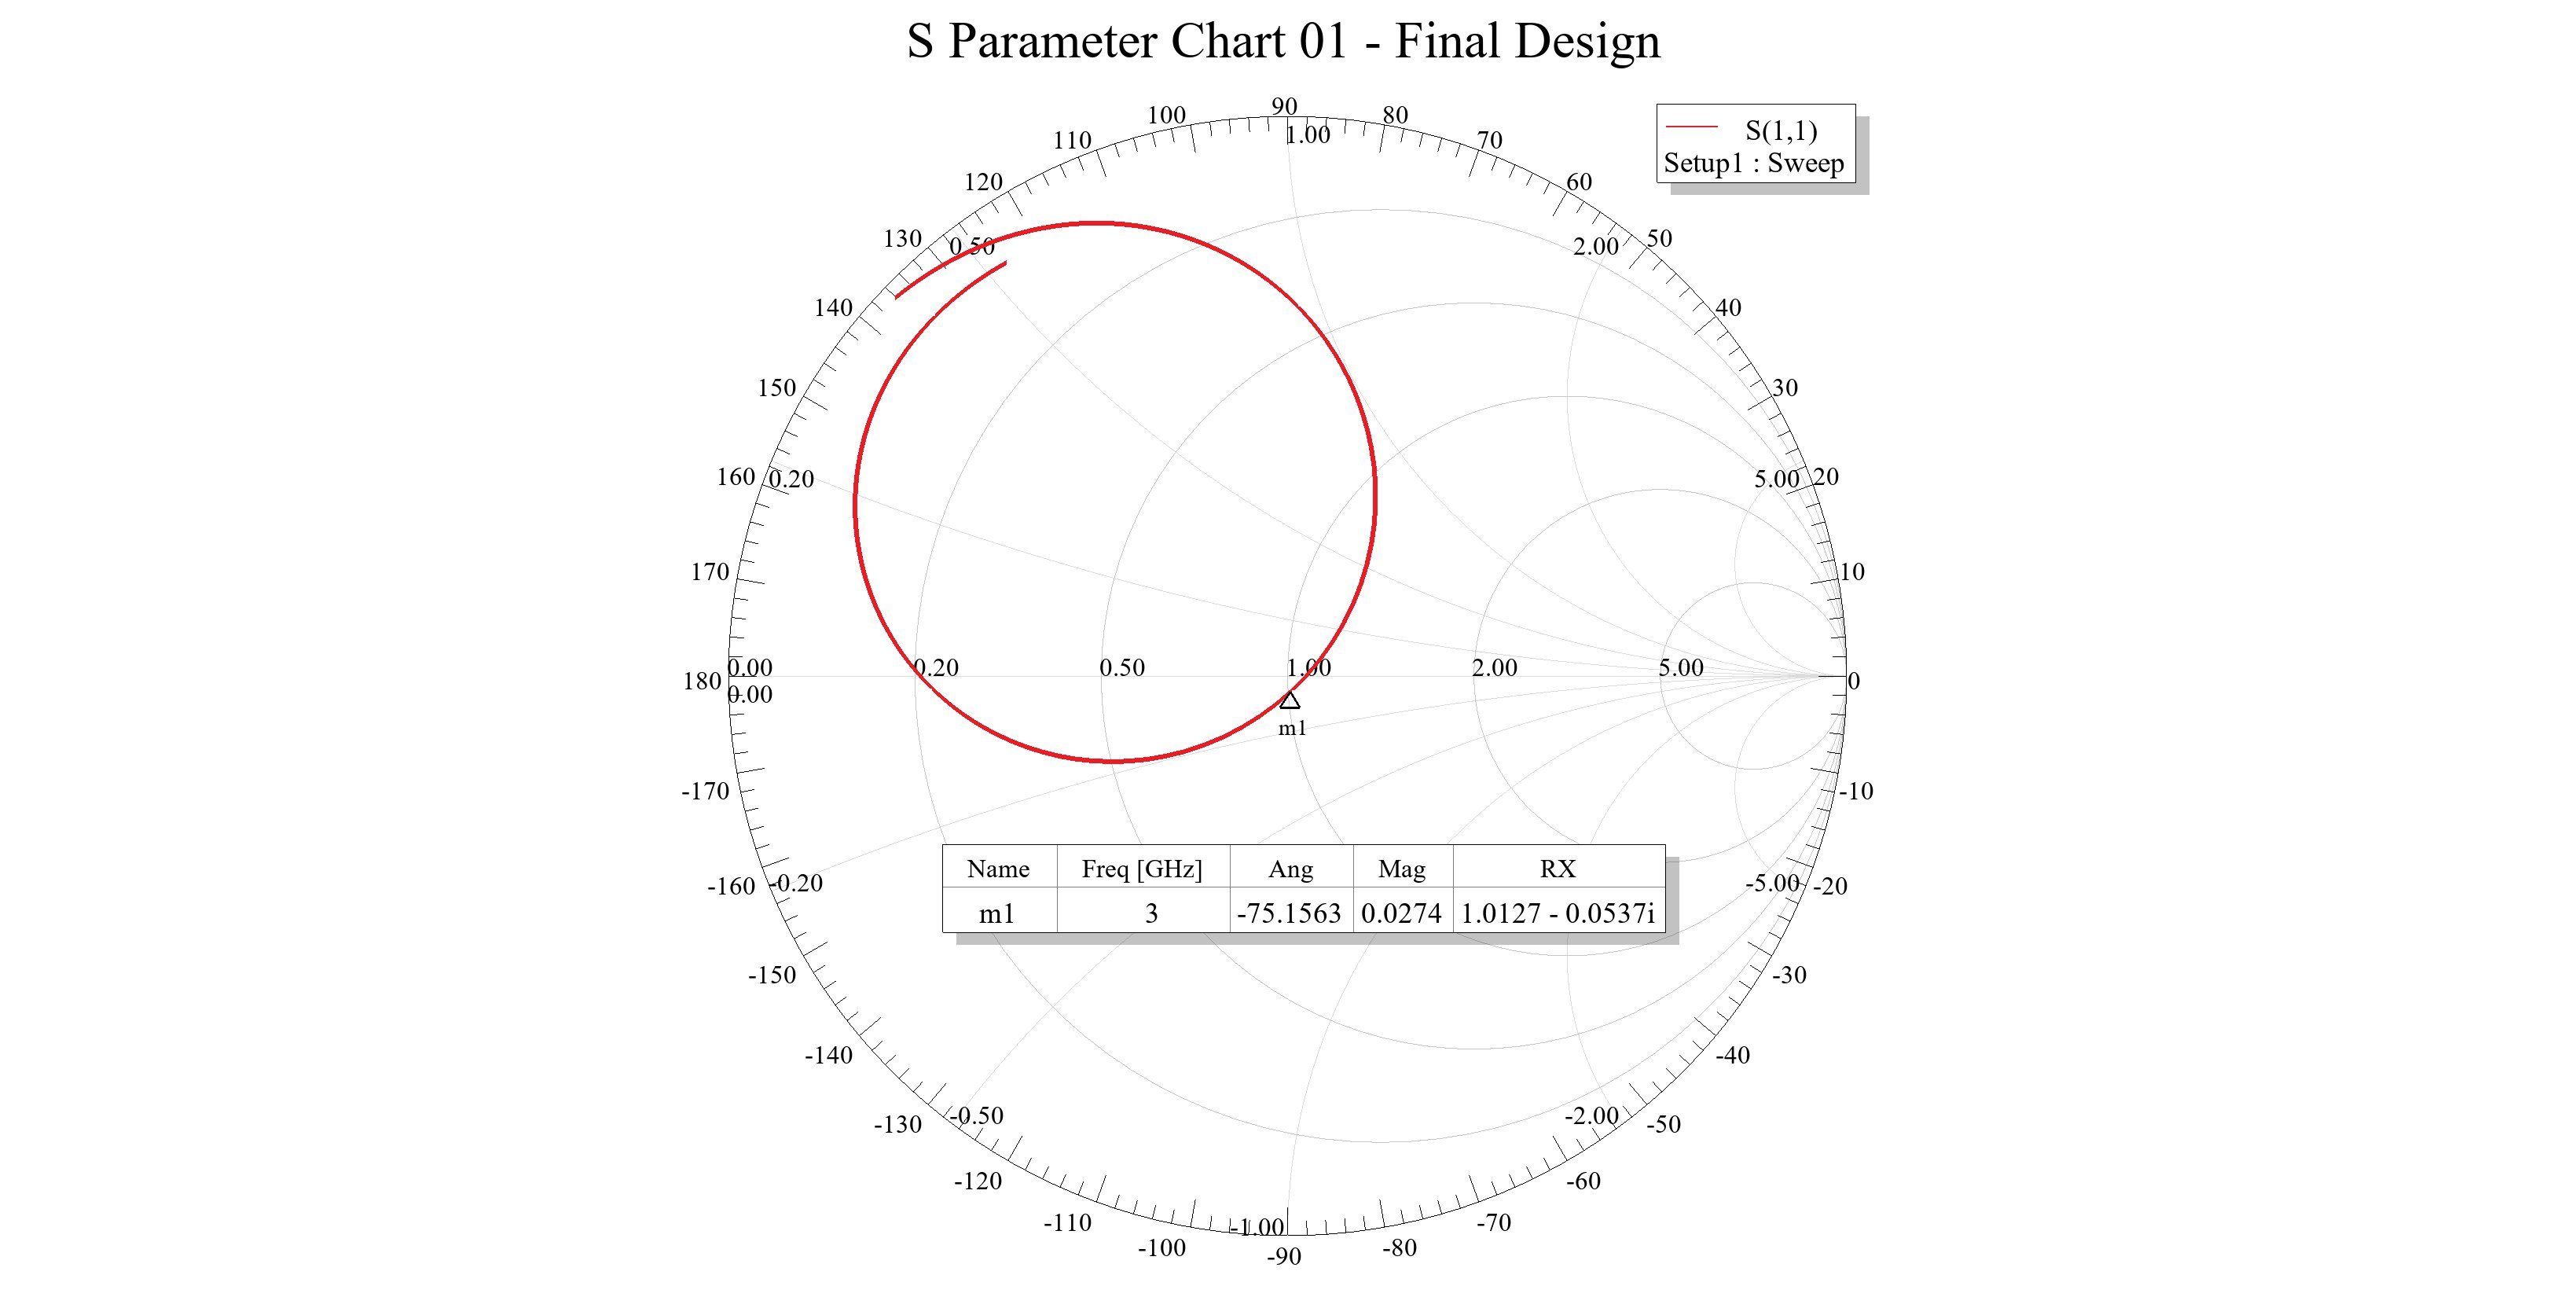
\includegraphics[width=0.875\textwidth,keepaspectratio,clip,trim=0.25cm 1.25cm 3.25cm 3.25cm]{img/S_Parameter_Chart_01___Final_Design_SmithCh.jpg}
        \caption{\small $|S_{11}|_\text{(dB)}$ design impedance from 2.5 to 3.5 GHz: demonstrates a good match at $3\,\text{GHz}$}
    \end{figure}
\end{frame}
\clearpage

\subsection[10~dB $\text{BW}_f$]{\texorpdfstring{$\text{BW}_f$ at \& $-10$~dB Points}{Bandwidth Plot: -10~dB Points}}
\begin{frame}
    \begin{figure}
        \centering
        \vspace*{-0.48cm}
        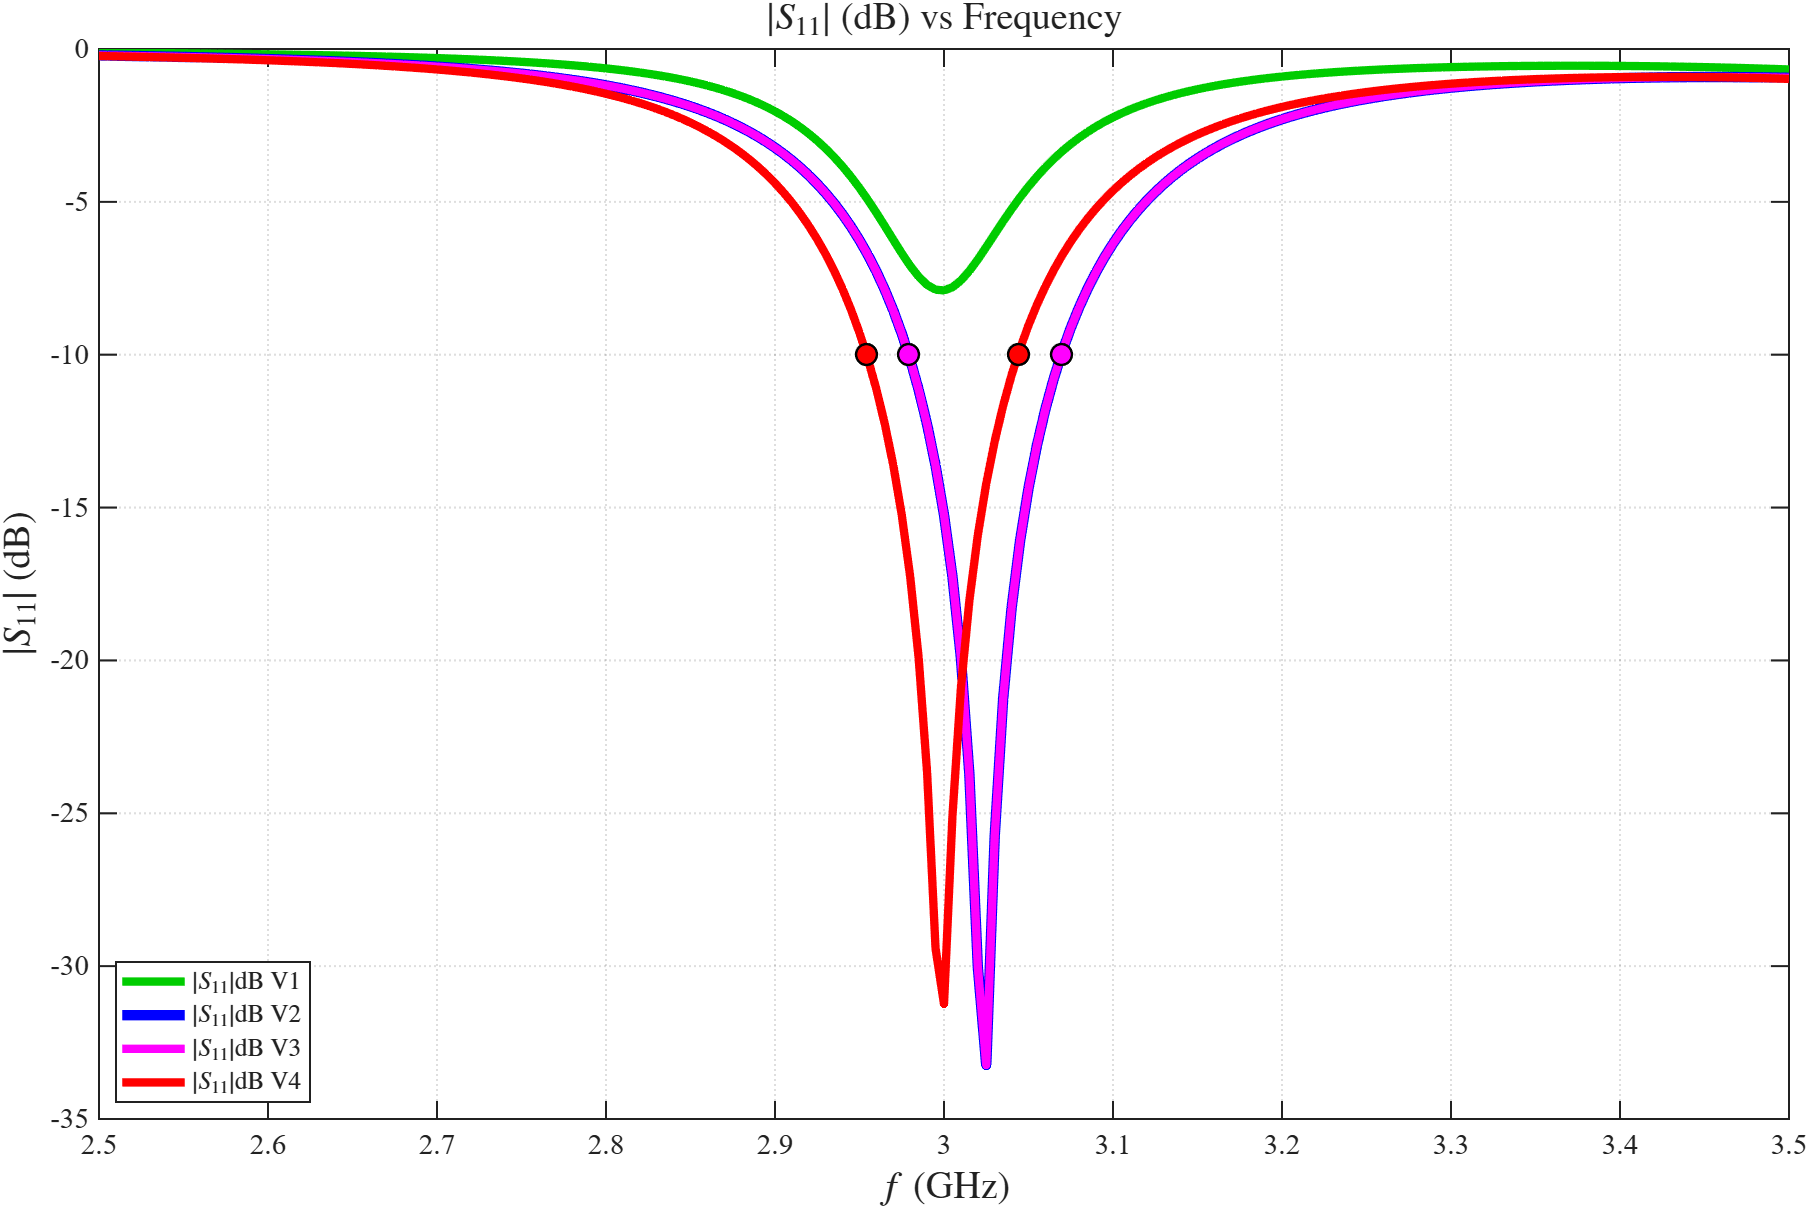
\includegraphics[width=0.65\textwidth,keepaspectratio,clip,trim=0cm 0.65cm 0cm 0.65cm]{img/Matlab_Figure_2_All_Sweeps_Matlab_10dB.png}
        \caption{$|S_{11}|$ (dB) vs $f$ (GHz) --- MATLAB plot of the $-10$~dB points, per optimetric sweep.}
    \end{figure}
\end{frame}

%%%%%%%%%%%%%%%%%%%%%%%%%%%%%%%%%%%%%%%%%%%%%%%%%%%%%%%%%%%%%%%%%%%%%%%%%%%%%%%%%%
% CONCLUSION
%%%%%%%%%%%%%%%%%%%%%%%%%%%%%%%%%%%%%%%%%%%%%%%%%%%%%%%%%%%%%%%%%%%%%%%%%%%%%%%%%%

\section[Conclusion]{Conclusion}

\subsection[Summary]{Summary}

\begin{frame}{Summary \& Conclusions}
    \textbf{Accomplishments:}
    \begin{enumerate}
        \item Successfully designed a 3-GHz coaxial-fed microstrip patch antenna
        \item Optimized feed position through parametric HFSS sweeps
        \item Achieved target $|S_{11}| \le -30$~dB at resonance
        \item Characterized E-plane and H-plane radiation patterns
    \end{enumerate}

    \vspace{1em}
    \textbf{Key Results:}
    \begin{itemize}
        \item Fractional bandwidth ($-10$~dB): $\sim 3\%$
        \item Final optimized dimensions validated through simulation
        \item Good impedance match demonstrated on Smith chart
    \end{itemize}
\end{frame}

%%%%%%%%%%%%%%%%%%%%%%%%%%%%%%%%%%%%%%%%%%%%%%%%%%%%%%%%%%%%%%%%%%%%%%%%%%%%%%%%%%
% APPENDICES OVERVIEW
%%%%%%%%%%%%%%%%%%%%%%%%%%%%%%%%%%%%%%%%%%%%%%%%%%%%%%%%%%%%%%%%%%%%%%%%%%%%%%%%%%

\section[Appendices]{Appendices}

\subsection[Appendix T.o.C.]{Table of Appendices}

\begin{frame}{Appendices}
    \footnotesize
    \begin{multicols}{2}
        \tableofcontents[sectionstyle=show/show,subsectionstyle=show/show,sections={8-11}]
    \end{multicols}
\end{frame}

%%%%%%%%%%%%%%%%%%%%%%%%%%%%%%%%%%%%%%%%%%%%%%%%%%%%%%%%%%%%%%%%%%%%%%%%%%%%%%%%%%
% APPENDIX
%%%%%%%%%%%%%%%%%%%%%%%%%%%%%%%%%%%%%%%%%%%%%%%%%%%%%%%%%%%%%%%%%%%%%%%%%%%%%%%%%%

\appendix

\section[HFSS Plots]{Appendix I -- HFSS Plots}
\subsection[V1]{\texorpdfstring{$|S_{11}|_\text{dB}$ vs $f$: Optimetric Sweep 01}{|S11| vs f: Optimetric Sweep 01}}
\begin{frame}
    \begin{figure}
        \centering
        \vspace*{-0.5cm}
        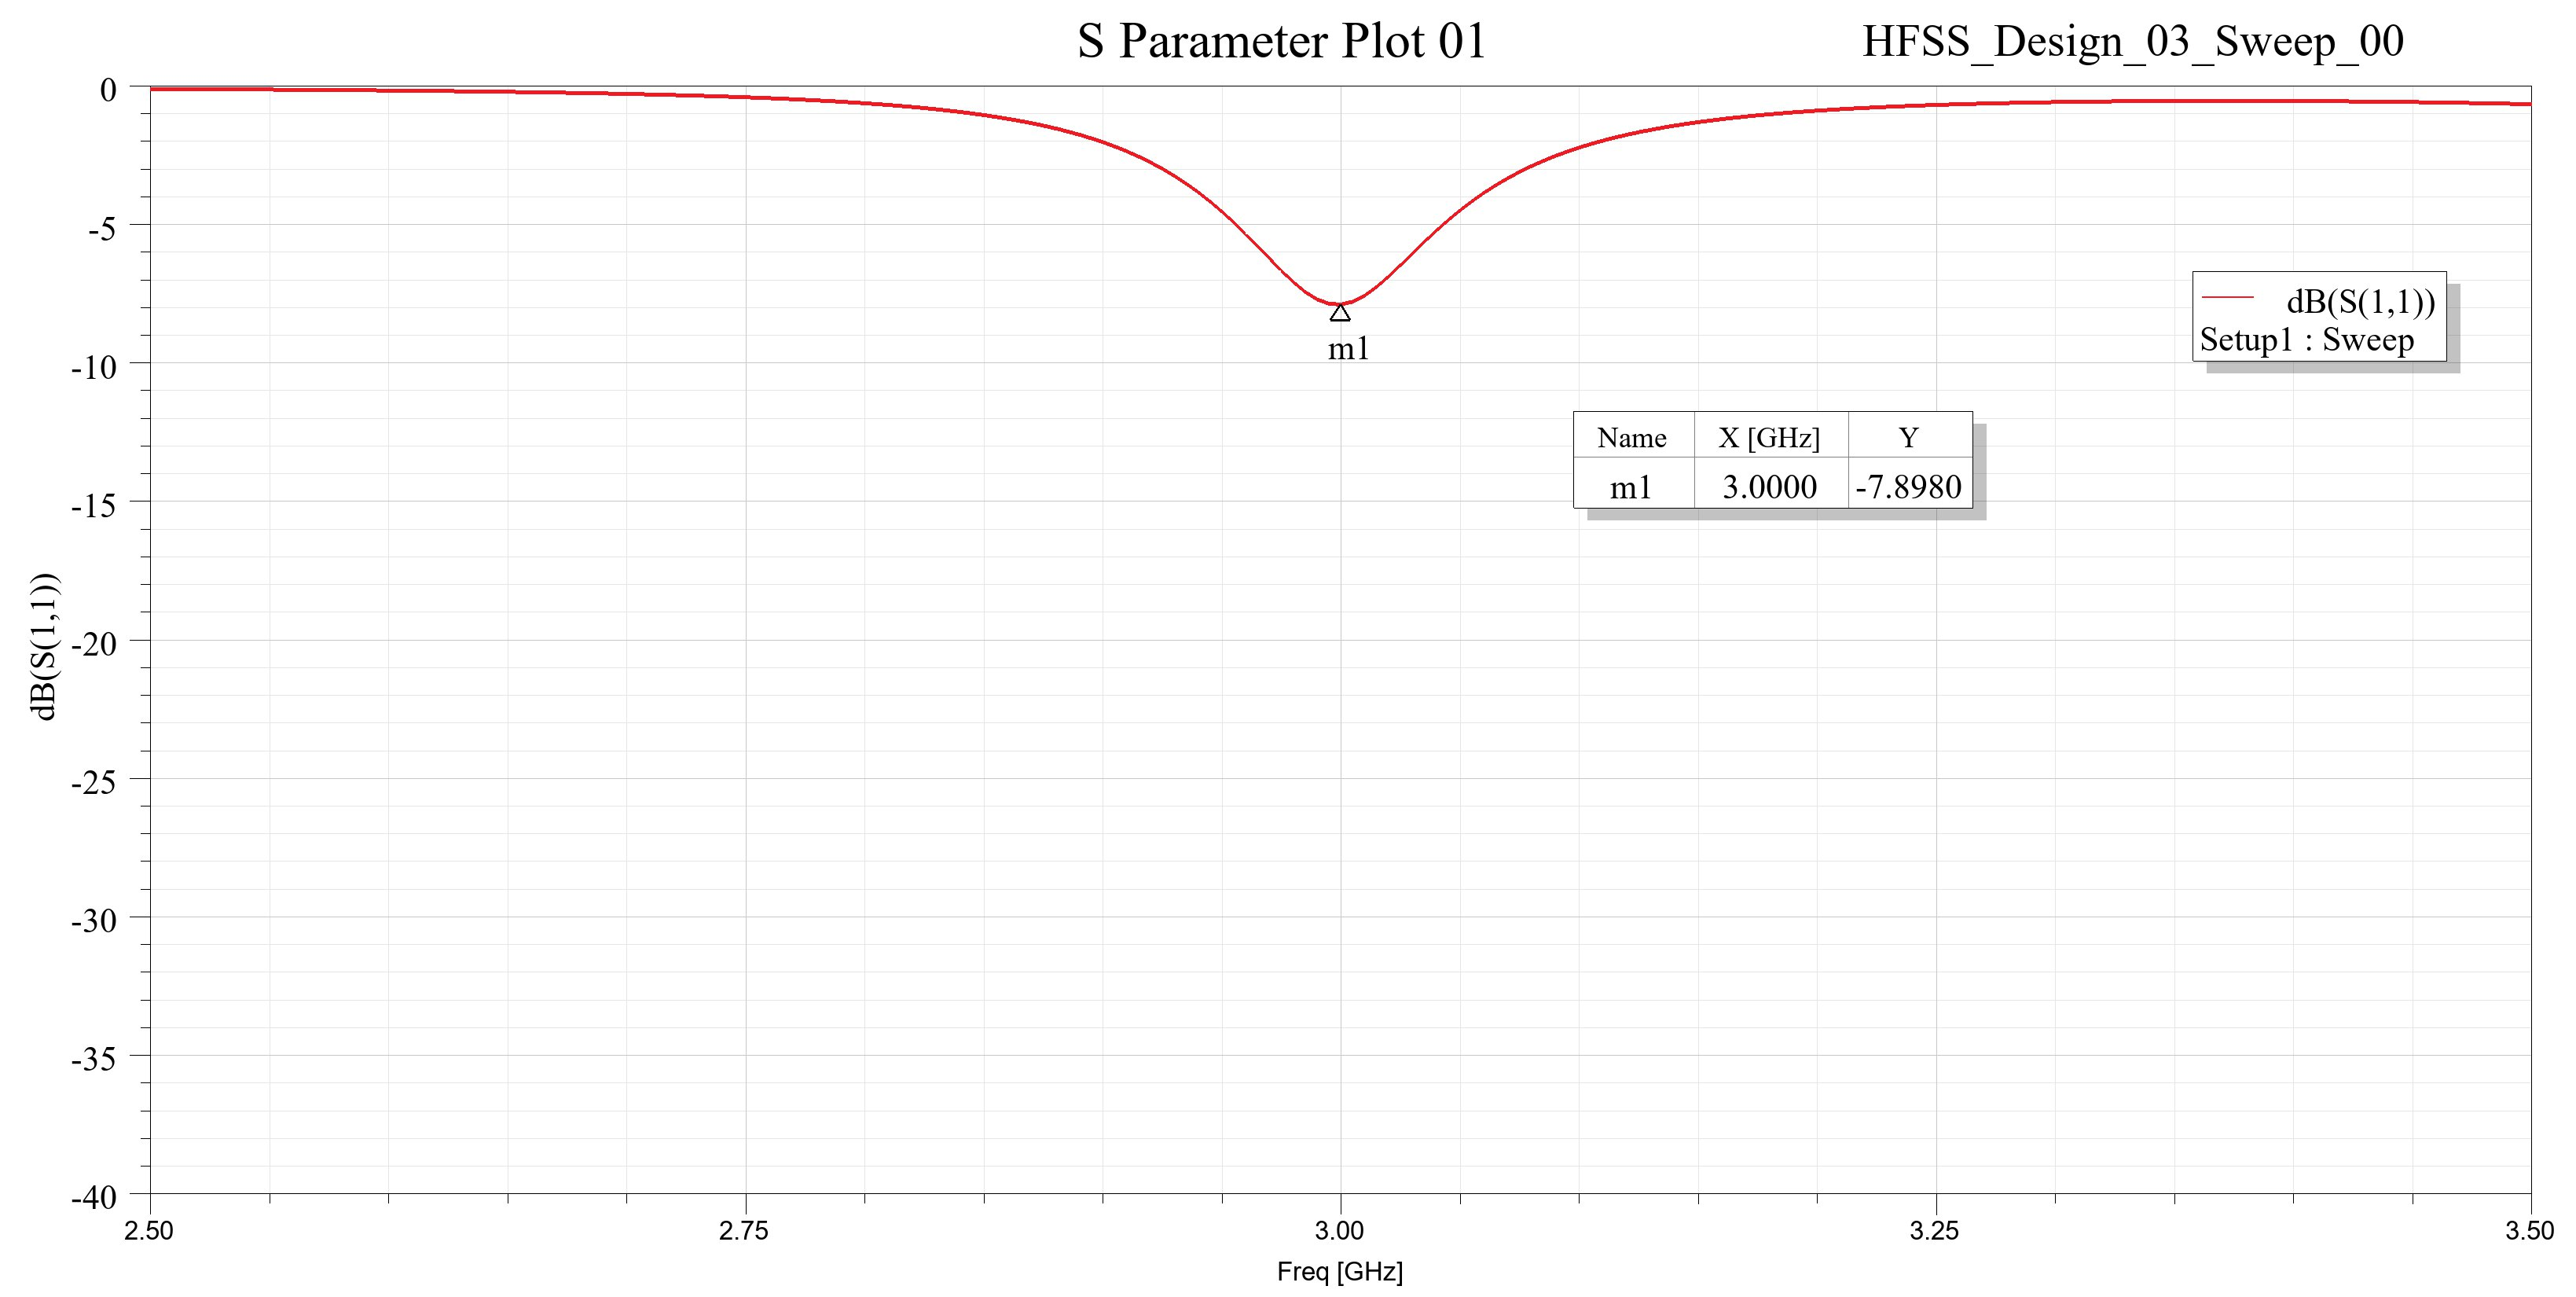
\includegraphics[width=0.8745\textwidth,keepaspectratio,clip,trim=0cm 0.05cm 0cm 2.65cm]{img/S_Parameter_Plot_01_Sweep_01.jpg}
        \caption{Optimetric Sweep V1: $|S_{11}|_\text{(dB)}$ vs $f_\text{(GHz)}$ (initial design).}
    \end{figure}
\end{frame}

\clearpage

\newpage
\subsection[V2 (All Traces)]{S-Parameters: Sweep 02 (All Traces)}
\begin{frame}
    \begin{figure}
        \centering
        \vspace*{-0.5cm}
        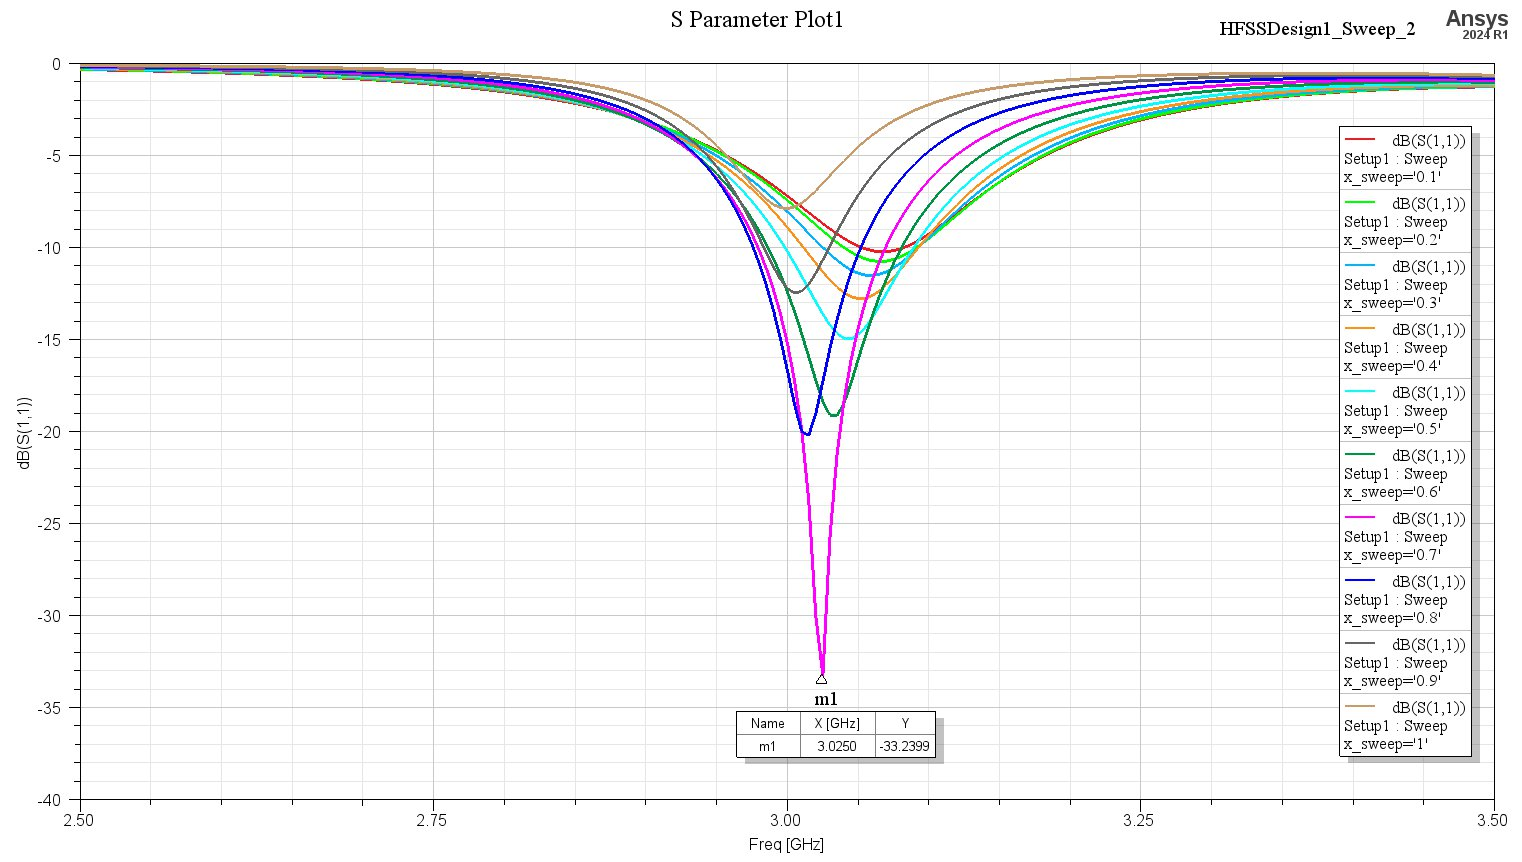
\includegraphics[width=0.857\textwidth,keepaspectratio,clip,trim=0cm 1.95cm 0cm 2.05cm]{img/S_Parameter_Plot_01___Sweep_02__All_Traces.jpg}
        \vspace*{-0.1cm}
        \caption{V2: All HFSS optimetric iterations for $X_{\text{sweep}}$. Linear frequency sweep from 2.5~GHz to 3.5~GHz with step $\Delta f = X_{\text{sweep}}/10$, spanning $X_{\text{sweep}}/10$ to $X_{\text{sweep}}$.}
    \end{figure}
\end{frame}

\clearpage

\newpage
\subsection[V2]{\texorpdfstring{V2: $|S_{11}|_\text{dB}$ vs $f_\text{()GHz)}$ V2 (Best Result)}{HFSS Plot |S(1,1)|dB for Sweep 02 (Best)}}
\begin{frame}
	\begin{figure}
		\centering
		\vspace*{-0.5cm}
		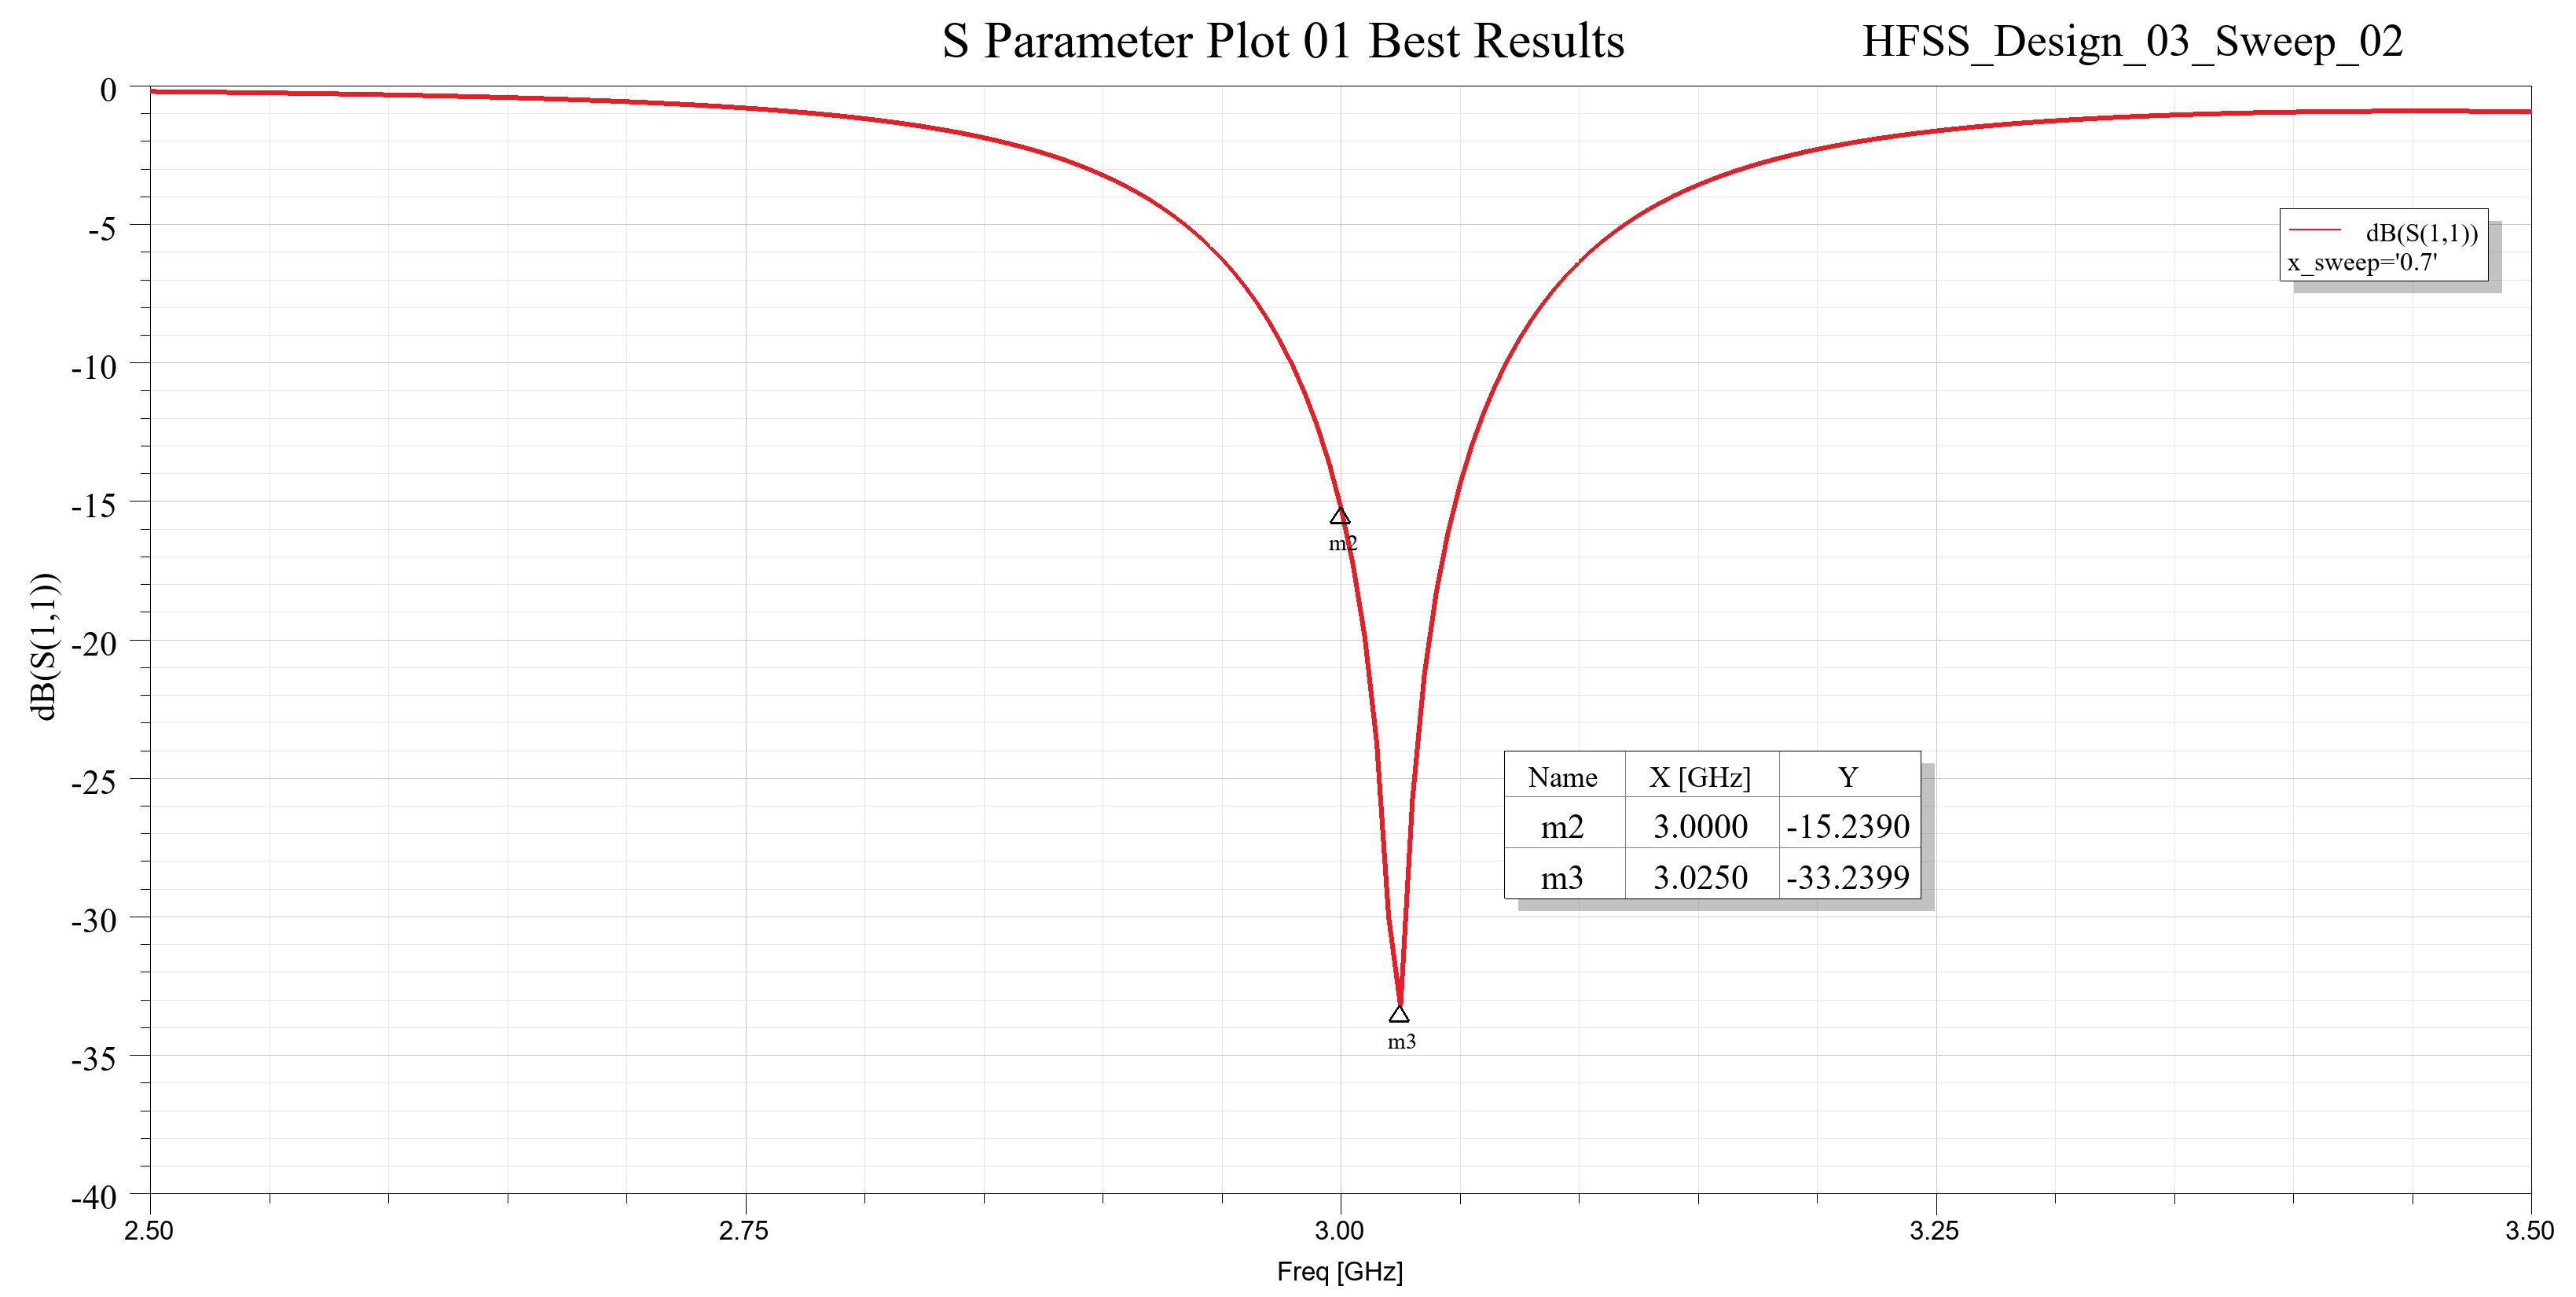
\includegraphics[width=0.8745\textwidth,keepaspectratio,clip,trim=0cm 1.0cm 0cm 3.1cm]{img/S_Parameter_Plot_01_Sweep_02.jpg}
		\vspace*{-0.05cm}
		\caption{\small HFSS Optimetric Sweep 02: Best result from optimetric Sweep 02}
	\end{figure}
\end{frame}

\subsection[Sweep 03]{S-Parameters: Sweep 03}
\begin{frame}
    \begin{figure}
        \centering
        \vspace*{-0.5cm}
        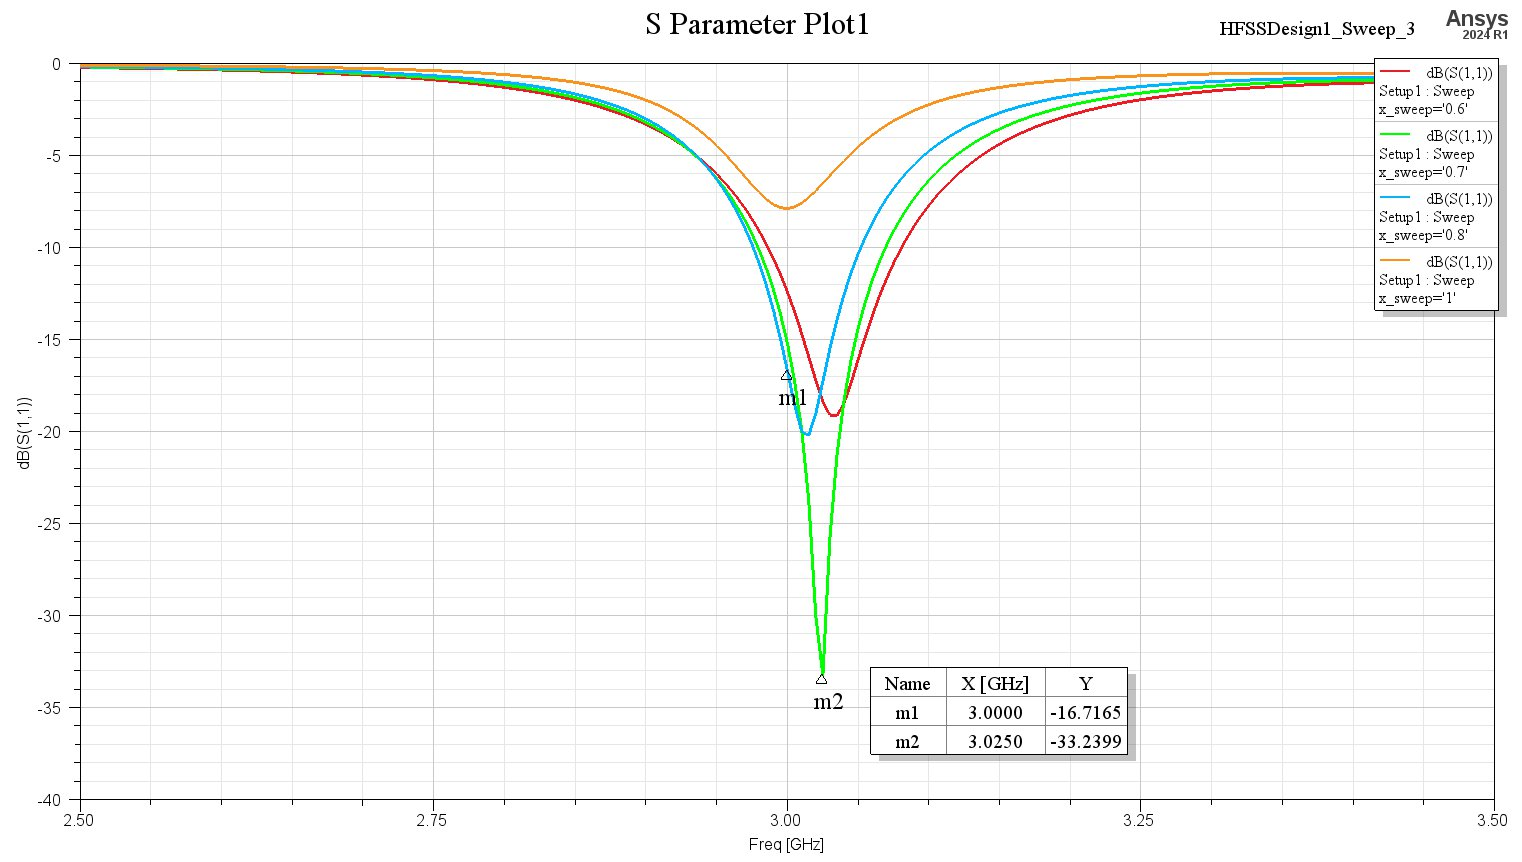
\includegraphics[width=0.85\textwidth,keepaspectratio,clip,trim=0cm 1.1925cm 0cm 1.975cm]{img/S_Parameter_Plot_01___Sweep_03.jpg}
        \vspace*{-0.05cm}
        \caption{S-Parameters: Sweep 03\newline $X_{\text{sweep}}$ with 0.02~GHz step refinement}
    \end{figure}
\end{frame}

\subsection[Sweep 03 (Refined)]{S-Parameters: Sweep 03 (Refined)}
\begin{frame}
    \begin{figure}
        \centering
        \vspace*{-0.5cm}
        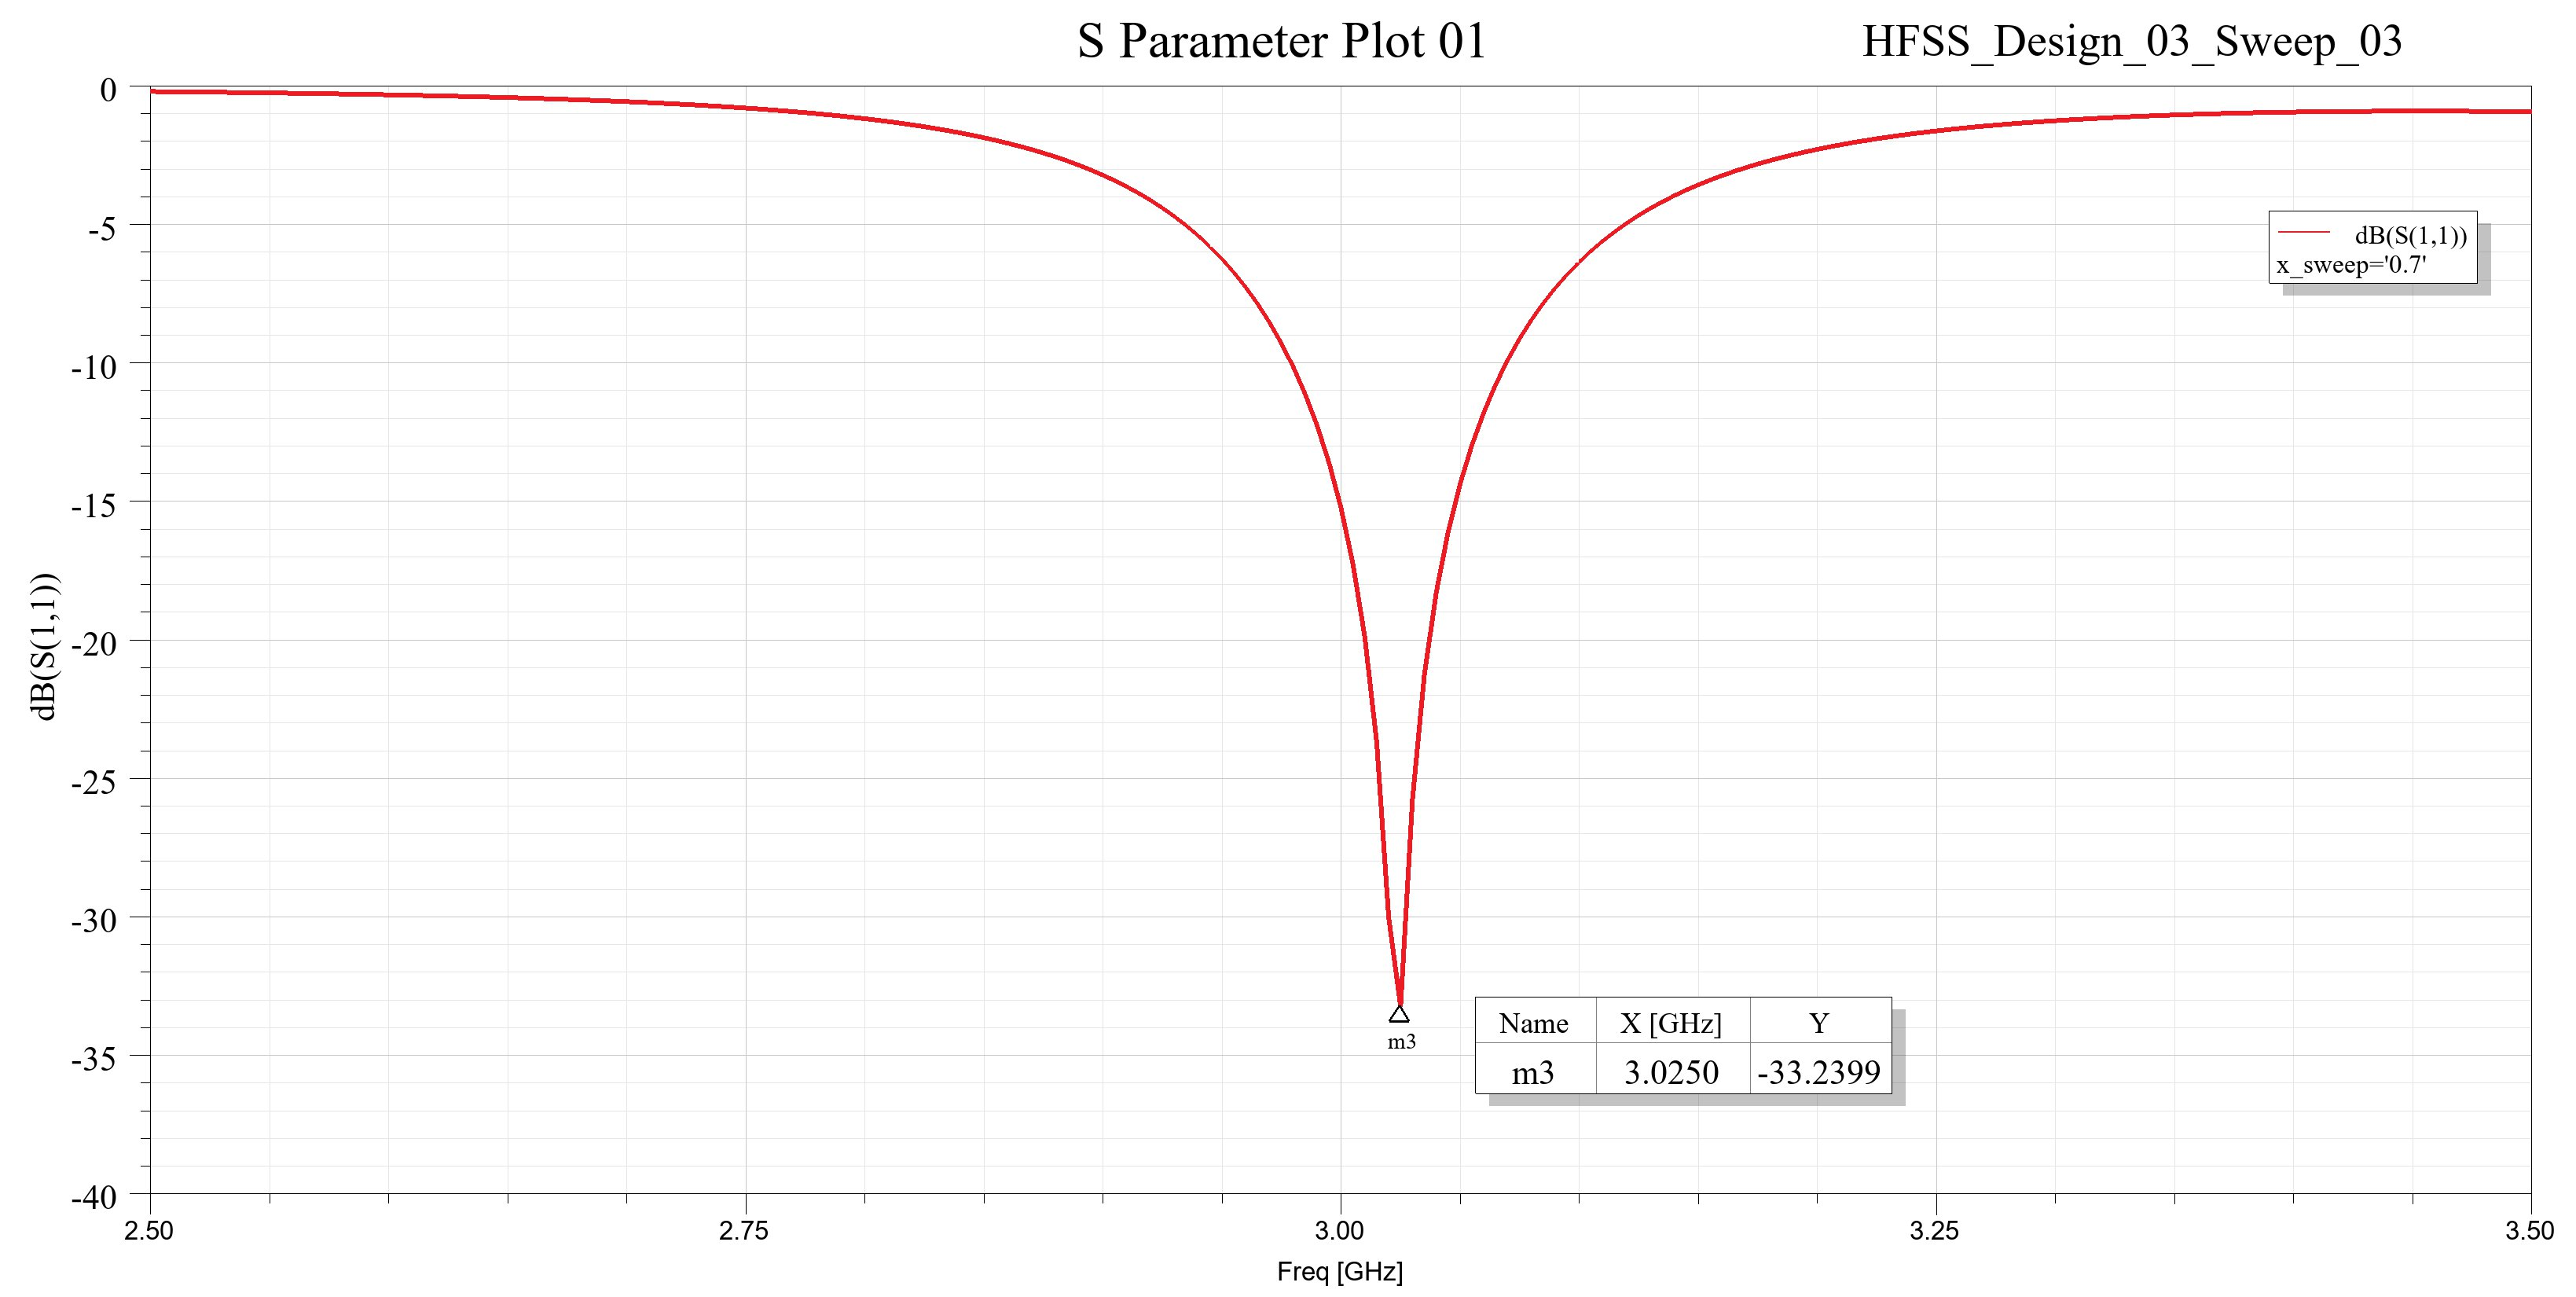
\includegraphics[width=0.85\textwidth,keepaspectratio,clip,trim=0cm 0.25cm 0cm 3.1cm]{img/S_Parameter_Plot_01_Sweep_03.jpg}
        \caption{S-Parameters: Sweep 03 (Refined)\newline Refined sweep focused near the resonance}
    \end{figure}
\end{frame}

\subsection[Sweep 04]{S-Parameters: Sweep 04}
\begin{frame}
    \begin{figure}
        \centering
        \vspace*{-0.5cm}
        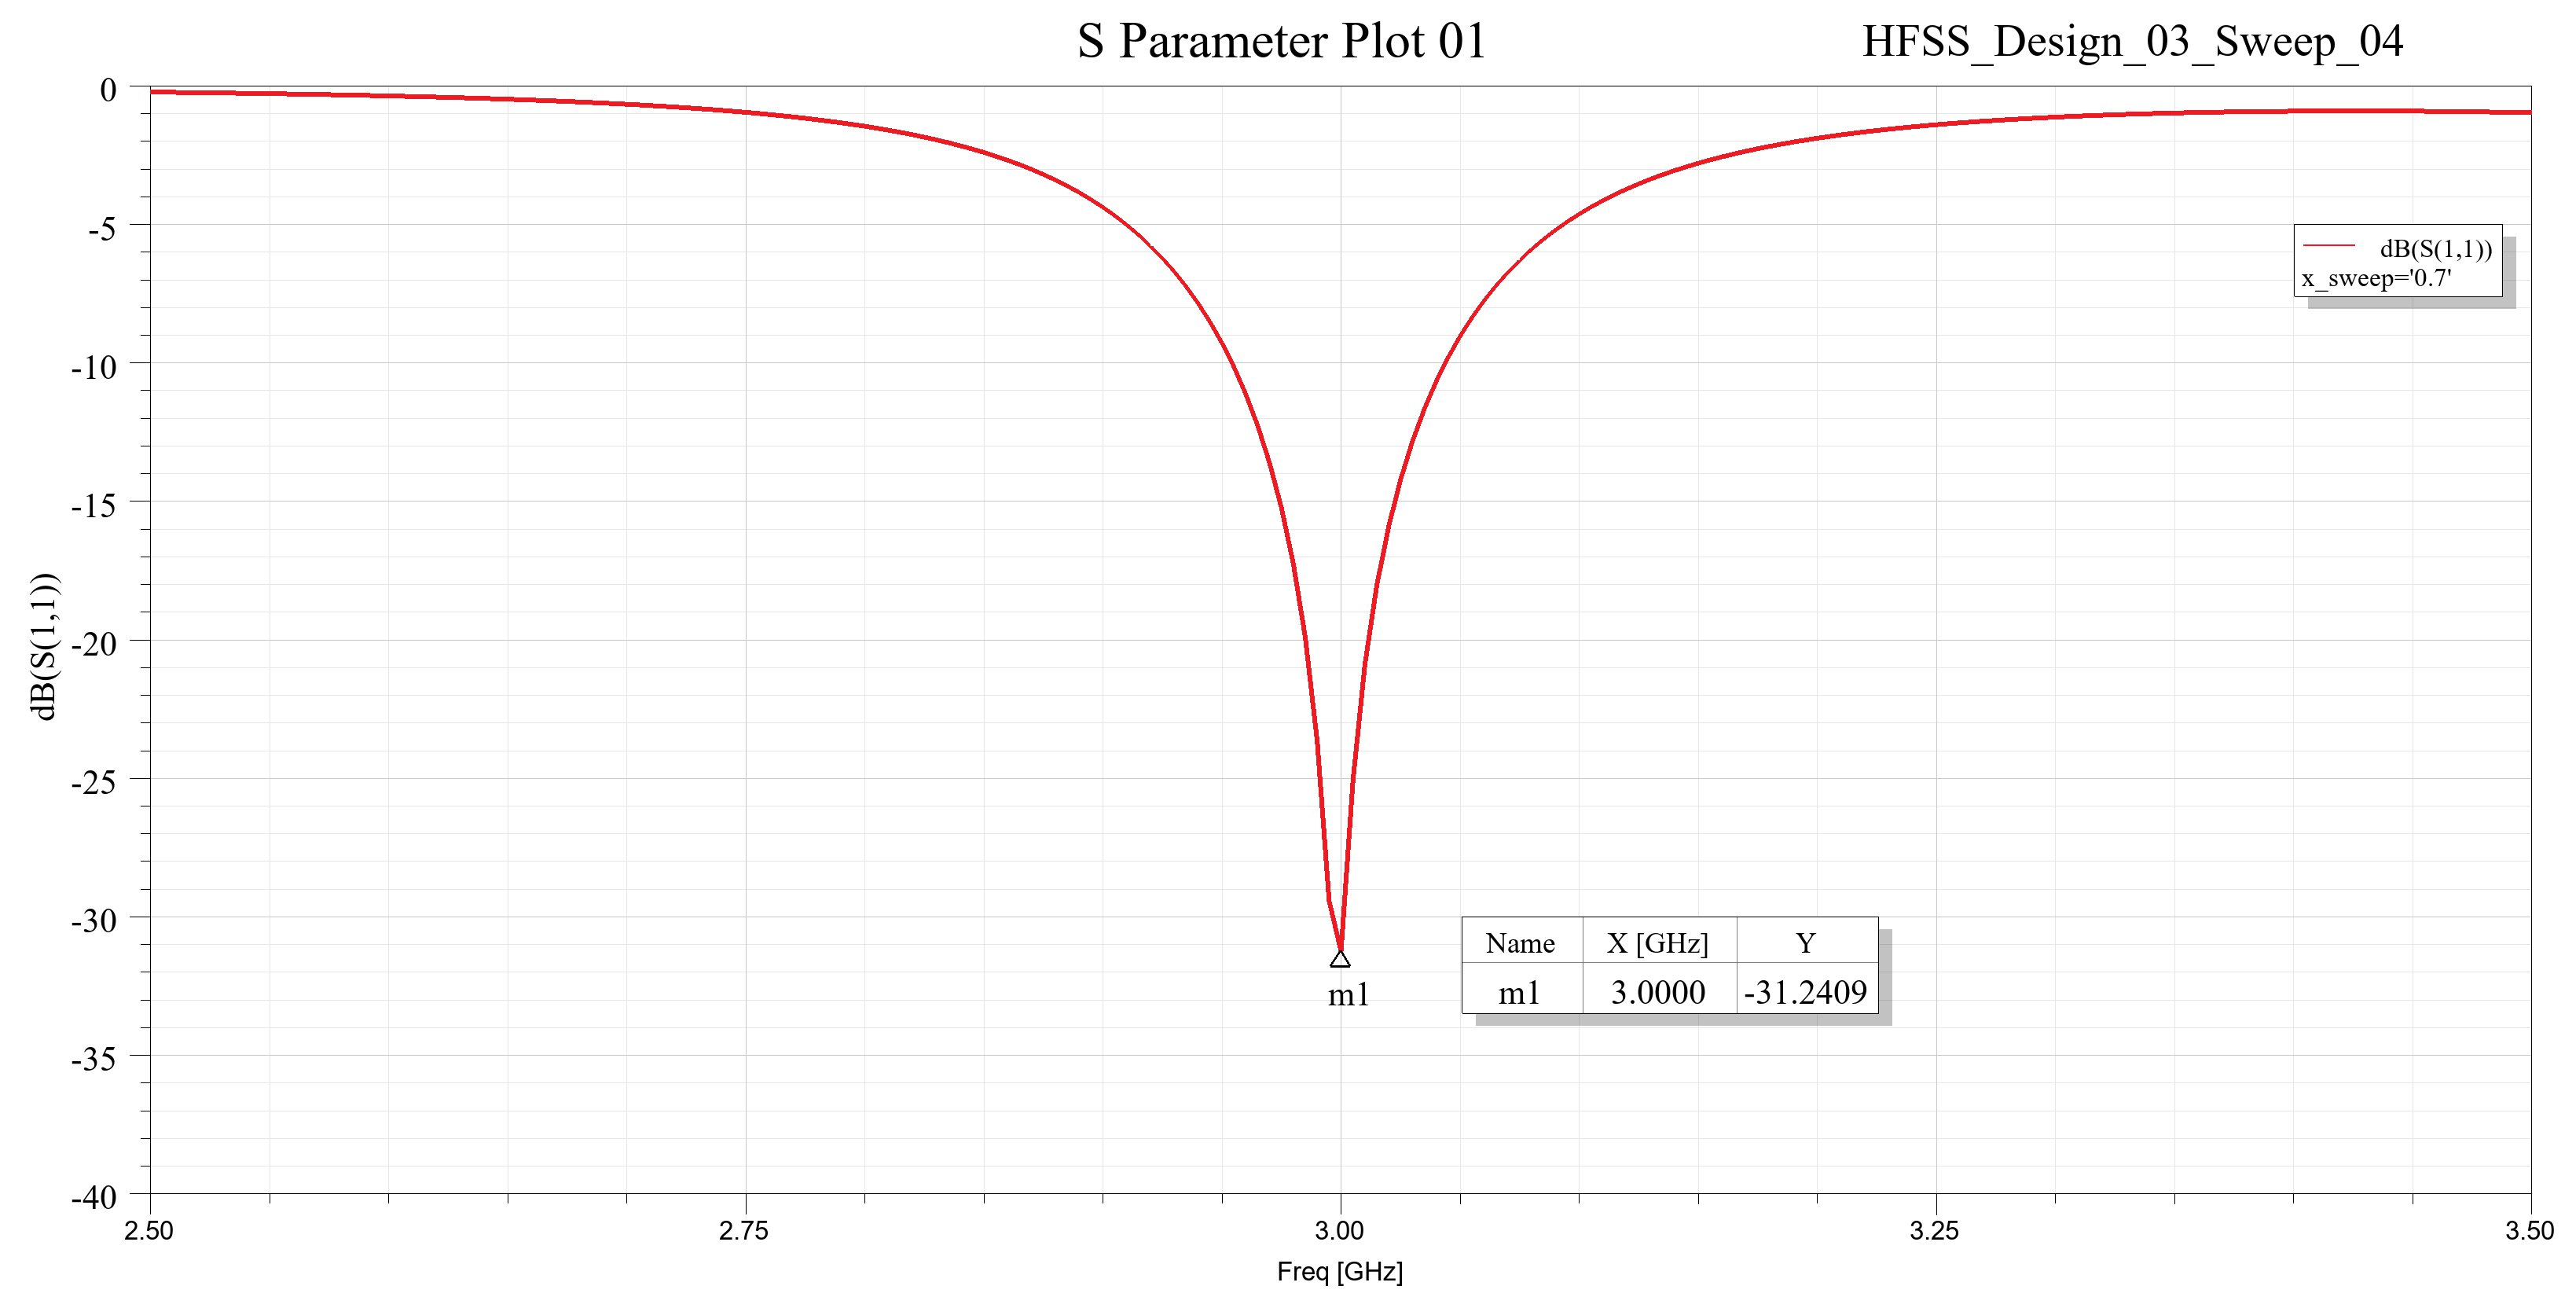
\includegraphics[width=0.85\textwidth,keepaspectratio,clip,trim=0cm 0.25cm 0cm 3.1cm]{img/S_Parameter_Plot_01_Sweep_04.jpg}
        \caption{S-Parameters: Sweep 04\newline Final optimized sweep for $|S_{11}|$}
    \end{figure}
\end{frame}

\section[MATLAB Code]{Appendix: MATLAB Code}

\ActivateVerbatimLigatures

%%%%%%%%%%%%%%%%%%%%%%%%%%%%%%%%%%%%%%%%%%%%%%%%%%%%%%%%%%%%%%%%%%%%%%%%%%%%%%%%%%
% APPENDIX I: MATLAB DESIGN CODE (two-column listings)
%%%%%%%%%%%%%%%%%%%%%%%%%%%%%%%%%%%%%%%%%%%%%%%%%%%%%%%%%%%%%%%%%%%%%%%%%%%%%%%%%%

\begin{frame}[fragile]{Appendix I: MATLAB Design Code}
    \begin{columns}[T]
        \begin{column}{0.49\textwidth}
\subsection[Design code 1]{EE\_457\_Design\_Project\_03\_Placzek\_Matlab.m (Lines 1--47)}
            \begin{lstlisting}
%% ------------------------------------------------------------------------
% EE_457_Design_Project_03_Placzek_Matlab.m
% Calculations and Design for EE-457 Design Project 03.
% Implements the transmission-line patch calculations for EE-457.
% IMPORTANT NOTE: This script relies on the presence of Dr. Burke's
% MATLAB_EELab/* MATLAB scripts in the MATLAB PATH in order to run.
% (e.g., EE457_Microstrip_Patch_Conductance).

clc; close all; clear all;

projDir = fileparts(mfilename('fullpath'));
rootDir = fileparts(projDir);
% eelabRoot = fullfile(rootDir, 'MATLAB_EELab');
% if exist(eelabRoot, 'dir') && ~contains(path, eelabRoot)
%     addpath(genpath(eelabRoot));
% else
%     warning('MATLAB_EELab path not found: %s', eelabRoot);
% end

%% ------------------------------------------------------------------------
% Input specifications

specs = defaultSpecs();

%% ------------------------------------------------------------------------
% Transmission-line design parameters

Dims = computeDimensions(specs);

%% ------------------------------------------------------------------------
% Edge conductance and feed offset (per EE457 helper)

Edge = computeEdgeQuantities(specs, Dims);
Feed = computeFeedLocation(specs, Dims, Edge);

%% ------------------------------------------------------------------------
% Performance expectations (HPBW heuristic & bandwidth estimate)

Pattern = estimatePattern(specs, Dims);
BW = estimateBandwidth(specs, Dims);

%% ------------------------------------------------------------------------
% Aggregate results, print summary, and write tables

Results = assembleResults(specs, Dims, Edge, Feed, Pattern, BW);
displaySummary(Results);
writeTables(Results);
            \end{lstlisting}
        \end{column}
        \begin{column}{0.49\textwidth}
\subsection[Design code 2]{EE\_457\_Design\_Project\_03\_Placzek\_Matlab.m (Lines 48--101)}
            \begin{lstlisting}[firstnumber=48]
%% ------------------------------------------------------------------------
% DEFAULTSPECS --> Project inputs and physical constants.

function specs = defaultSpecs()
specs.f0 = 3e9;                % Hz
specs.h = 1.5748e-3;           % m (62 mil)
specs.er = 4.4;                % FR-4 εr
specs.tand = 0.02;             % Loss tangent (documentation)
specs.t_patch = 18e-6;         % Copper thickness (m)
specs.rin = 50;                % Target input resistance (ohm)
specs.widthFactor = 1.5;       % W ~=~ 1.5 * Le (assignment requirement)
specs.substrateFactor = 1.5;   % Ls ~=~ Ws ~=~ 1.5 × patch size
specs.c0 = 299792458;
specs.lambda0 = specs.c0/specs.f0;
specs.k0 = 2*pi/specs.lambda0;
specs.eta0 = 376.730313668;
end

%% ------------------------------------------------------------------------
% computeDimensions --> Does exactly what it sounds like it would do.

function dims = computeDimensions(specs)
lambda_g = specs.lambda0/sqrt(specs.er);      % Guided λ using ε_r
Le = 0.5 * lambda_g;
W = specs.widthFactor * Le;                   % Physical patch width

eps_eff = effectivePermittivity(specs, W);
deltaL = fringingExtension(specs, W, eps_eff);
L = Le - 2*deltaL;
Ls = specs.substrateFactor * L;
Ws = specs.substrateFactor * W;

lambda_g_eff = specs.lambda0/sqrt(eps_eff);   % Useful for documentation.

Dims = struct(); %#ok<NASGU>
dims.lambda_g = lambda_g;
dims.lambda_g_eff = lambda_g_eff;
dims.Le = Le;
dims.W = W;
dims.Wprime = W;
dims.eps_eff = eps_eff;
dims.deltaL = deltaL;
dims.L = L;
dims.Ls = Ls;
dims.Ws = Ws;
end

%%-------------------------------------------------------------------------
% Hammerstad Expression

function eps_eff = effectivePermittivity(specs, W) % Hammerstad expression.
ratio = specs.h/max(W, 1e-12);
eps_eff = (specs.er + 1)/2 + (specs.er - 1)/2 * (1 + 12*ratio)^(-0.5);
end
            \end{lstlisting}
        \end{column}
    \end{columns}
\end{frame}

\begin{frame}[fragile]{Appendix I: MATLAB Design Code (cont.)}
    \begin{columns}[T]
        \begin{column}{0.49\textwidth}
\subsection[Design code 3]{EE\_457\_Design\_Project\_03\_Placzek\_Matlab.m (Lines 102--147)}
            \begin{lstlisting}[firstnumber=102]
%%-------------------------------------------------------------------------
% FRINGINGEXTENSION -> Hammerstad extension length on one side.
function deltaL = fringingExtension(specs, W, eps_eff)
ratio = W/specs.h;
deltaL = 0.412*specs.h * ((eps_eff + 0.3)*(ratio + 0.264))/((eps_eff - 0.258)*(ratio + 0.8));
end

%% COMPUTEEDGEQUANTITIES -> Calls the EE457 conductance helper script.
function edge = computeEdgeQuantities(specs, dims)
[Gedge, G1, G12, B1, G1a, B1a] = EE457_Microstrip_Patch_Conductance( ...
    dims.Le, dims.W, specs.h, specs.k0, specs.lambda0, specs.eta0);
edge.Gedge = Gedge;
edge.G1 = G1;
edge.G12 = G12;
edge.B1 = B1;
edge.G1_approx = G1a;
edge.B1_approx = B1a;
edge.Redge = 1/Gedge;
end

%% COMPUTEFEEDLOCATION --> Coaxial probe distance from radiating edge.
function feed = computeFeedLocation(specs, dims, edge)
ratio = min(max(specs.rin/edge.Redge, 0), 1);
xf = (dims.Le/pi) * acos(sqrt(ratio));
x0 = 0.5*dims.Le - xf;
feed.xf = xf;
feed.x0 = x0;
feed.Rin = specs.rin;
end

%% ESTIMATEPATTERN --> Coarse HPBW/directivity expectated values.
function pattern = estimatePattern(specs, dims)
lambda_g = dims.lambda_g;
BWE = 50 * (lambda_g/dims.L);
BWH = 50 * (lambda_g/dims.W);
BWE = min(max(BWE, 30), 180);
BWH = min(max(BWH, 30), 180);
Dlin = 41253/(BWE * BWH);
Ddb = 10*log10(Dlin);
pattern.BWE = BWE;
pattern.BWH = BWH;
pattern.Dlin = Dlin;
pattern.DdB = Ddb;
pattern.Glin = Dlin;
pattern.GdB = Ddb;
end
            \end{lstlisting}
        \end{column}
        \begin{column}{0.49\textwidth}
\subsection[Design code 4]{EE\_457\_Design\_Project\_03\_Placzek\_Matlab.m (Lines 148--192)}
            \begin{lstlisting}[firstnumber=148]
%% ------------------------------------------------------------------------
%  ESTIMATEBANDWIDTH --> -10 dB impedance bandwidth (transmission-line Q).

function bw = estimateBandwidth(specs, dims)
er = specs.er;
h = specs.h;
lambda0 = specs.lambda0;
fracBW = 3.77 * ((er - 1)/(er^2)) * (h/lambda0);
VSWR = 1.92; % -10 dB return-loss circle
fracBW = fracBW * sqrt((VSWR - 1)/VSWR);
bw.abs = fracBW * specs.f0;
bw.frac = fracBW;
bw.percent = fracBW * 100;
end

%% ------------------------------------------------------------------------
%  ASSEMBLERESULTS --> Organizes script output values for console and CSV.

function results = assembleResults(specs, dims, edge, feed, pattern, bw)
mm = 1e-3;
um = 1e-6;
results.f0_GHz = specs.f0/1e9;
results.h_mm = specs.h/mm;
results.er = specs.er;
results.lambda_g_mm = dims.lambda_g/mm;
results.Le_mm = dims.Le/mm;
results.Wprime_mm = dims.Wprime/mm;
results.eps_eff = dims.eps_eff;
results.deltaL_um = dims.deltaL/um;
results.L_mm = dims.L/mm;
results.W_mm = dims.W/mm;
results.Redge_ohm = edge.Redge;
results.xf_mm = feed.xf/mm;
results.x0_mm = feed.x0/mm;
results.Ls_mm = dims.Ls/mm;
results.Ws_mm = dims.Ws/mm;
results.BWE_deg = pattern.BWE;
results.BWH_deg = pattern.BWH;
results.D_lin = pattern.Dlin;
results.D_dB = pattern.DdB;
results.G_lin = pattern.Glin;
results.G_dB = pattern.GdB;
results.BW_MHz = bw.abs/1e6;
results.BW_percent = bw.percent;
end
            \end{lstlisting}
        \end{column}
    \end{columns}
\end{frame}

\begin{frame}[fragile]{Appendix I: MATLAB Design Code (cont.)}
    \begin{columns}[T]
        \begin{column}{0.49\textwidth}
\subsection[Design code 5]{EE\_457\_Design\_Project\_03\_Placzek\_Matlab.m (Lines 193--206)}
            \begin{lstlisting}[firstnumber=193]
%% ------------------------------------------------------------------------
%  DISPLAYSUMMARY --> Print concise summary for sanity checks.

function displaySummary(results)
fprintf('--- EE-457 Design Project 03: Table 01 Calculations --\n');
fprintf('\nf0 = %.4f GHz\n\nεr = %.4f\n\nh = %.4f mm\n', results.f0_GHz, results.er, results.h_mm);
fprintf('\nλg = %.4f mm\n\nLe = %.4f mm\n\nW = %.4f mm\n\nL = %.4f mm\n', ...
        results.lambda_g_mm, results.Le_mm, results.W_mm, results.L_mm);
fprintf('\nΔL = %.4f µm\n\nR_edge = %.4f Ω\n\nxf = %.4f mm (from edge)\n', ...
        results.deltaL_um, results.Redge_ohm, results.xf_mm);
fprintf('\nHPBW_E = %.4f°\n\nHPBW_H = %.4f°\n\nD ≈ %.4f (%.4f dB)\n', ...
        results.BWE_deg, results.BWH_deg, results.D_lin, results.D_dB);
fprintf('\nEstimated BW10dB = %.4f MHz (%.4f%%)\n', results.BW_MHz, results.BW_percent);
end
            \end{lstlisting}
        \end{column}
        \begin{column}{0.49\textwidth}
\subsection[Design code 6]{EE\_457\_Design\_Project\_03\_Placzek\_Matlab.m (Lines 207--225)}
            \begin{lstlisting}[firstnumber=207]
%% ------------------------------------------------------------------------
%  WRITETABLES --> Populate calculated columns for Tables 1 and 4.

function writeTables(results)
rootDir = fileparts(mfilename('fullpath'));
tablesDir = fullfile(rootDir, 'tables');
if ~exist(tablesDir, 'dir')
    mkdir(tablesDir);
end
T1 = table(results.f0_GHz, results.h_mm, results.er, results.lambda_g_mm, ...
    results.Le_mm, results.Wprime_mm, results.eps_eff, results.deltaL_um, ...
    results.L_mm, results.W_mm, results.Redge_ohm, results.xf_mm, ...
    'VariableNames', {'f0_GHz','h_mm','eps_r','lambda_g_mm','Le_mm','Wprime_mm', ...
                      'eps_eff','deltaL_um','L_mm','W_mm','R_edge_ohm','xf_mm'});
writetable(T1, fullfile(tablesDir, 'table_1_calculated.csv'));
T4 = table(results.BW_MHz, results.BW_percent, ...
    'VariableNames', {'BW_10dB_MHz','BW_10dB_percent'});
writetable(T4, fullfile(tablesDir, 'table_4_calculated.csv'));
end
            \end{lstlisting}
        \end{column}
    \end{columns}
\end{frame}

%%%%%%%%%%%%%%%%%%%%%%%%%%%%%%%%%%%%%%%%%%%%%%%%%%%%%%%%%%%%%%%%%%%%%%%%%%%%%%%%%%
% APPENDIX II: MATLAB -10 dB BANDWIDTH CODE (two-column listings)
%%%%%%%%%%%%%%%%%%%%%%%%%%%%%%%%%%%%%%%%%%%%%%%%%%%%%%%%%%%%%%%%%%%%%%%%%%%%%%%%%%

\begin{frame}[fragile]{Appendix II: MATLAB $-10$~dB Bandwidth Code}
    \begin{columns}[T]
        \begin{column}{0.49\textwidth}
\subsection[$-10$ dB code 1]{EE\_457\_Design\_Project\_03\_Placzek\_Matlab\_read\_csv\_10dB.m (Lines 1--29)}
            \begin{lstlisting}
% EE_457_Design_Project_03_Placzek_Matlab_read_csv_10dB.m
% Matlab script for creating |S11|dB versus frequency plots
% Uses all *.csv files in the current project directory.
% Assumptions (HFSS-style export):
%  - Each CSV file has at least three columns:
%      Col 1: sweep variable (ignored here)
%      Col 2: frequency (GHz by default; see PlotSpec.freqInHz)
%      Col 3: |S11| in dB
%  - Files are named so that alphabetical sort produces V1, V2, V3, V4, ...
% Behavior:
%  - All traces are plotted on a single figure.
%  - All traces get -10 dB markers at crossings.
%  - A -10 dB bandwidth is computed and printed for each trace (BW_f),
%     or reported as N/A if there are fewer than two -10 dB crossings.

clc; close all; clear all;

projDir = fileparts(mfilename('fullpath')); %#ok<NASGU>

%% ------------------------------------------------------------------------
%  Plot configuration and file discovery

PlotSpec = default_Plot_Spec();
files = list_Csv_Files(pwd);                % Use current working directory

%% ------------------------------------------------------------------------
%  Generate S11 plot

Fig = plot_All_S11(files, PlotSpec); %#ok<NASGU>
            \end{lstlisting}
        \end{column}
        \begin{column}{0.49\textwidth}
\subsection[$-10$ dB code 2]{EE\_457\_Design\_Project\_03\_Placzek\_Matlab\_read\_csv\_10dB.m (Lines 30--71)}
            \begin{lstlisting}[firstnumber=30]
%% ------------------------------------------------------------------------
%  DEFAULT_PLOT_SPEC --> Styles and options for S11 plotting.

function PlotSpec = default_Plot_Spec()
PlotSpec = struct();
PlotSpec.colorList = [
    0.0  0.8  0.0;   % V1  - green
    0.0  0.0  1.0;   % V2  - blue
    1.0  0.0  1.0;   % V3  - magenta
    1.0  0.0  0.0;   % V4  - red
];
PlotSpec.lineWidths = [4 5 4 4];
PlotSpec.markerLevel_dB = -10;        % Level for bandwidth markers (dB)
PlotSpec.markerIndices  = [];         % [] => mark all traces
PlotSpec.lineWidth      = 3;          % fallback if lineWidths not used
PlotSpec.markerSize     = 10;
PlotSpec.fontSizeAxes   = 14;
PlotSpec.fontSizeLabel  = 18;
PlotSpec.fontSizeLegend = 12;
PlotSpec.fontName       = 'Times New Roman';
PlotSpec.gridLineStyle  = ':';
PlotSpec.gridLineWidth  = 1;
PlotSpec.titleString = '$|S_{11}|$ (dB) vs Frequency';
PlotSpec.legendStrings = { ...
    '$|S_{11}|$dB V1', ...
    '$|S_{11}|$dB V2', ...
    '$|S_{11}|$dB V3', ...
    '$|S_{11}|$dB V4'};
PlotSpec.freqInHz = false;            % Set true if CSV frequency is in Hz
end

%% ------------------------------------------------------------------------
%  LIST_CSV_FILES --> Find and alphabetize all *.csv files in a directory.

function files = list_Csv_Files(dirPath)
files = dir(fullfile(dirPath, '*.csv'));
if isempty(files)
    error('No .csv files found in directory: %s', dirPath);
end
[~, idx] = sort({files.name});
files = files(idx);
end
            \end{lstlisting}
        \end{column}
    \end{columns}
\end{frame}

\begin{frame}[fragile]{Appendix II: MATLAB $-10$~dB Bandwidth Code (cont.)}
    \begin{columns}[T]
        \begin{column}{0.49\textwidth}
\subsection[$-10$ dB code 3]{EE\_457\_Design\_Project\_03\_Placzek\_Matlab\_read\_csv\_10dB.m (Lines 72--125)}
            \begin{lstlisting}[firstnumber=72]
%% ------------------------------------------------------------------------
%  PLOT_ALL_S11 --> Read CSVs, plot all |S11| curves, and decorate axes.

function Fig = plot_All_S11(files, PlotSpec)
Fig = figure; hold on; grid on; box on;
set(Fig, 'Color', 'w');
nFiles   = numel(files);
nColors  = size(PlotSpec.colorList, 1);
fprintf('--- %.1f dB bandwidths from |S_{11}| ---\n', ...
        abs(PlotSpec.markerLevel_dB));
for k = 1:nFiles
    filePath = fullfile(files(k).folder, files(k).name);
    [f, s11] = read_S11_Trace(filePath, PlotSpec.freqInHz);
    if isempty(f) || numel(s11) < 2
        warning('Skipping file with insufficient data: %s', files(k).name);
        continue;
    end
    c = PlotSpec.colorList(min(k, nColors), :);
    name = strip_Extension(files(k).name);
    if isfield(PlotSpec, 'lineWidths') && ~isempty(PlotSpec.lineWidths)
        lwList = PlotSpec.lineWidths;
        lw = lwList(min(k, numel(lwList)));
    else
        lw = PlotSpec.lineWidth;
    end
    plot(f, s11, ...                                                  % Main curve
        'LineWidth', lw, ...
        'Color', c, ...
        'DisplayName', name);
    markThisCurve = isempty(PlotSpec.markerIndices) || ...
                    ismember(k, PlotSpec.markerIndices);
    bw = computeBandwidthFromLevel(f, s11, PlotSpec.markerLevel_dB);  % -10 dB crossings and bandwidth
    if markThisCurve && ~isempty(bw.crossings)
        plot(bw.crossings, ...
             PlotSpec.markerLevel_dB * ones(size(bw.crossings)), 'o', ...
             'MarkerFaceColor', c, ...
             'MarkerEdgeColor', 'k', ...
             'MarkerSize', PlotSpec.markerSize, ...
             'LineWidth', 1.2, ...
             'HandleVisibility', 'off');
    end
    if ~isnan(bw.BWabs)
        fprintf('%s: f0 ≈ %.4f GHz, ', name, bw.f0);
        fprintf('f_low = %.4f GHz, f_high = %.4f GHz, ', ...
                bw.fLow, bw.fHigh);
        fprintf('BW_f = %.4f GHz (%.4f%%)\n', ...
                bw.BWabs, bw.BWpercent);
    else
        fprintf('%s: BW_f = N/A (no %.1f dB crossings).\n', ...
                name, PlotSpec.markerLevel_dB);
    end
end
formatS11Axes(PlotSpec);
end
            \end{lstlisting}
        \end{column}
        \begin{column}{0.49\textwidth}
\subsection[$-10$ dB code 4]{EE\_457\_Design\_Project\_03\_Placzek\_Matlab\_read\_csv\_10dB.m (Lines 126--174)}
            \begin{lstlisting}[firstnumber=126]
%% ------------------------------------------------------------------------
%  READ_S11_TRACE --> Load frequency and |S11| from a CSV file.

function [f, s11] = read_S11_Trace(filePath, freqInHz)
T = readtable(filePath, 'PreserveVariableNames', true);
vars = T.Properties.VariableNames;
freqIdx = find(contains(vars, 'Freq', 'IgnoreCase', true), 1, 'first');
s11Idx  = find(contains(vars, 'dB',   'IgnoreCase', true) | ...
               contains(vars, 'S11',  'IgnoreCase', true), 1, 'first');
if isempty(freqIdx) || isempty(s11Idx)
    warning('Could not find frequency/S11 columns in %s. Skipping.', filePath);
    f   = [];
    s11 = [];
    return;
end
f   = T{:, freqIdx};                      % Extract numeric data
s11 = T{:, s11Idx};
bad = ~isfinite(f) | ~isfinite(s11);      % Drop any NaNs
f(bad)   = [];
s11(bad) = [];
if numel(f) < 2 || numel(s11) < 2         % Still not enough samples? bail.
    f   = [];
    s11 = [];
    return;
end
if freqInHz                               % Optional Hz → GHz conversion
    f = f/1e9;
end
end

%% ------------------------------------------------------------------------
%  LEVELCROSSINGS --> Linear interpolation for y = level crossings.

function crossings = levelCrossings(f, y, level)
delta    = y - level;
idxCross = find(delta(1:end-1) .* delta(2:end) <= 0);
crossings = zeros(size(idxCross));
for n = 1:numel(idxCross)
    i  = idxCross(n);
    f1 = f(i);    f2 = f(i+1);
    y1 = y(i);    y2 = y(i+1);

    if y2 ~= y1
        crossings(n) = f1 + (level - y1) * (f2 - f1) / (y2 - y1);
    else
        crossings(n) = f1;
    end
end
end
            \end{lstlisting}
        \end{column}
    \end{columns}
\end{frame}

\begin{frame}[fragile]{Appendix II: MATLAB $-10$~dB Code (cont.)}
    \begin{columns}[T]
        \begin{column}{0.49\textwidth}
\subsection[$-10$ dB code 5]{EE\_457\_Design\_Project\_03\_Placzek\_Matlab\_read\_csv\_10dB.m (Lines 175--208)}
            \begin{lstlisting}[firstnumber=175]
%% ------------------------------------------------------------------------
%  COMPUTEBANDWIDTHFROMLEVEL --> -10dB bandwidth around the resonance.

function bw = computeBandwidthFromLevel(f, s11, level_dB)
bw = struct();                                % Initialize struct with NaNs
bw.f0        = NaN;
bw.fLow      = NaN;
bw.fHigh     = NaN;
bw.BWabs     = NaN;
bw.BWfrac    = NaN;
bw.BWpercent = NaN;
bw.crossings = [];
if numel(f) < 2 || numel(s11) < 2
    return;
end
crossings = levelCrossings(f, s11, level_dB);
if numel(crossings) < 2
    return;
end
[~, idxMin] = min(s11);
f0    = f(idxMin);
fLow  = crossings(1);
fHigh = crossings(end);
BWabs     = fHigh - fLow;
BWfrac    = BWabs / f0;
BWpercent = 100 * BWfrac;
bw.f0        = f0;
bw.fLow      = fLow;
bw.fHigh     = fHigh;
bw.BWabs     = BWabs;
bw.BWfrac    = BWfrac;
bw.BWpercent = BWpercent;
bw.crossings = crossings;
end
            \end{lstlisting}
        \end{column}
        \begin{column}{0.49\textwidth}
\subsection[$-10$ dB code 6]{EE\_457\_Design\_Project\_03\_Placzek\_Matlab\_read\_csv\_10dB.m (Lines 209--240)}
            \begin{lstlisting}[firstnumber=209]
%% ------------------------------------------------------------------------
%  FORMAT_S11_AXES --> Publication-style axis, labels, and legend.

function formatS11Axes(PlotSpec)
set(gca, ...
    'FontSize', PlotSpec.fontSizeAxes, ...
    'FontName', PlotSpec.fontName, ...
    'GridLineStyle', PlotSpec.gridLineStyle, ...
    'LineWidth', PlotSpec.gridLineWidth);
xlabel('$f$ (GHz)', 'Interpreter', 'latex', ...
    'FontSize', PlotSpec.fontSizeLabel);
ylabel('$|S_{11}|$ (dB)', 'Interpreter', 'latex', ...
    'FontSize', PlotSpec.fontSizeLabel);
title(PlotSpec.titleString, 'Interpreter', 'latex', ... % Title
    'FontSize', PlotSpec.fontSizeLabel);
if isfield(PlotSpec, 'legendStrings') && ~isempty(PlotSpec.legendStrings)
    legend(PlotSpec.legendStrings, ...
        'Interpreter', 'latex', ...
        'Location', 'southwest', ...
        'FontSize', PlotSpec.fontSizeLegend);
else
    legend('show', 'Location', 'southwest', ...
        'FontSize', PlotSpec.fontSizeLegend);
end
end

%% ------------------------------------------------------------------------
%  STRIP_EXTENSION --> Remove file extension from a filename.

function name = strip_Extension(filename)
[~, name, ~] = fileparts(filename);
end
            \end{lstlisting}
        \end{column}
    \end{columns}
\end{frame}
%%%%%%%%%%%%%%%%%%%%%%%%%%%%%%%%%%%%%%%%%%%%%%%%%%%%%%%%%%%%%%%%%%%%%%%%%%%%%%%%%%
%%%%%%%%%%%%%%%%%%%%%%%%%%%%%%%%%%%%%%%%%%%%%%%%%%%%%%%%%%%%%%%%%%%%%%%%%%%%%%%%%%
% APPENDIX III: HFSS SCREENSHOTS
%%%%%%%%%%%%%%%%%%%%%%%%%%%%%%%%%%%%%%%%%%%%%%%%%%%%%%%%%%%%%%%%%%%%%%%%%%%%%%%%%%

\begin{frame}{Appendix III: HFSS Parameter Values}
    \begin{figure}
        \centering
        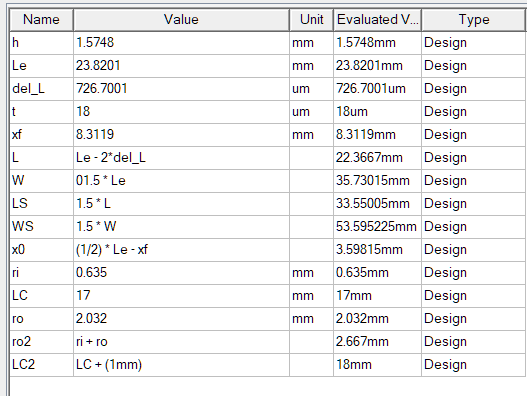
\includegraphics[width=0.82\textwidth,height=0.65\textheight,keepaspectratio]{img/sweep_00_values.png}
        \caption{Sweep 00 (Initial)}
        \label{fig:sweep00-values}
    \end{figure}
\end{frame}

\begin{frame}{Appendix III: HFSS Parameter Values (cont.)}
    \begin{figure}
        \centering
        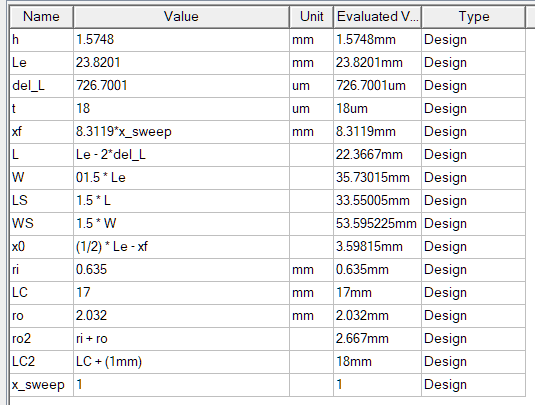
\includegraphics[width=0.82\textwidth,height=0.65\textheight,keepaspectratio]{img/sweep_01_values.png}
        \caption{Sweep 01}
        \label{fig:sweep01-values}
    \end{figure}
\end{frame}

\begin{frame}{Appendix III: HFSS Parameter Values (cont.)}
    \begin{figure}
        \centering
        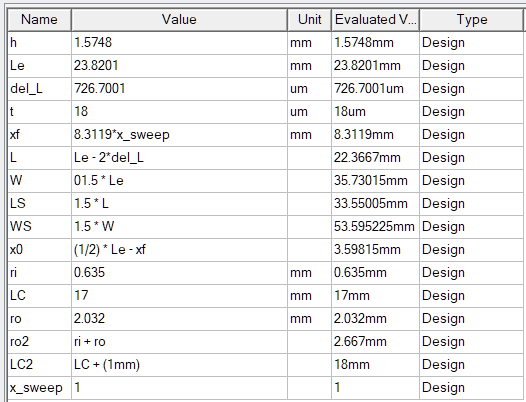
\includegraphics[width=0.82\textwidth,height=0.65\textheight,keepaspectratio]{img/sweep_03_values.png}
        \caption{Sweep 03}
        \label{fig:sweep03-values}
    \end{figure}
\end{frame}

\begin{frame}{Appendix III: HFSS Parameter Values (cont.)}
    \begin{figure}
        \centering
        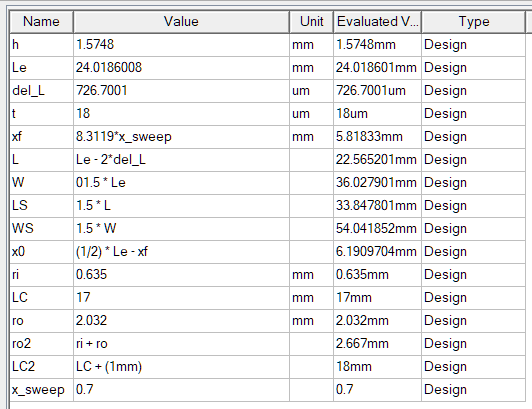
\includegraphics[width=0.82\textwidth,height=0.65\textheight,keepaspectratio]{img/sweep_04_values.png}
        \caption{Sweep 04}
        \label{fig:sweep04-values}
    \end{figure}
\end{frame}

\subsection[3~dB $\text{BW}_f$ Plot]{\texorpdfstring{MATLAB Plot of $\text{BW}_f$ at $-3$~dB}{MATLAB Plot of BW\_f at -3 dB}}
\begin{frame}
    \begin{figure}
        \centering
        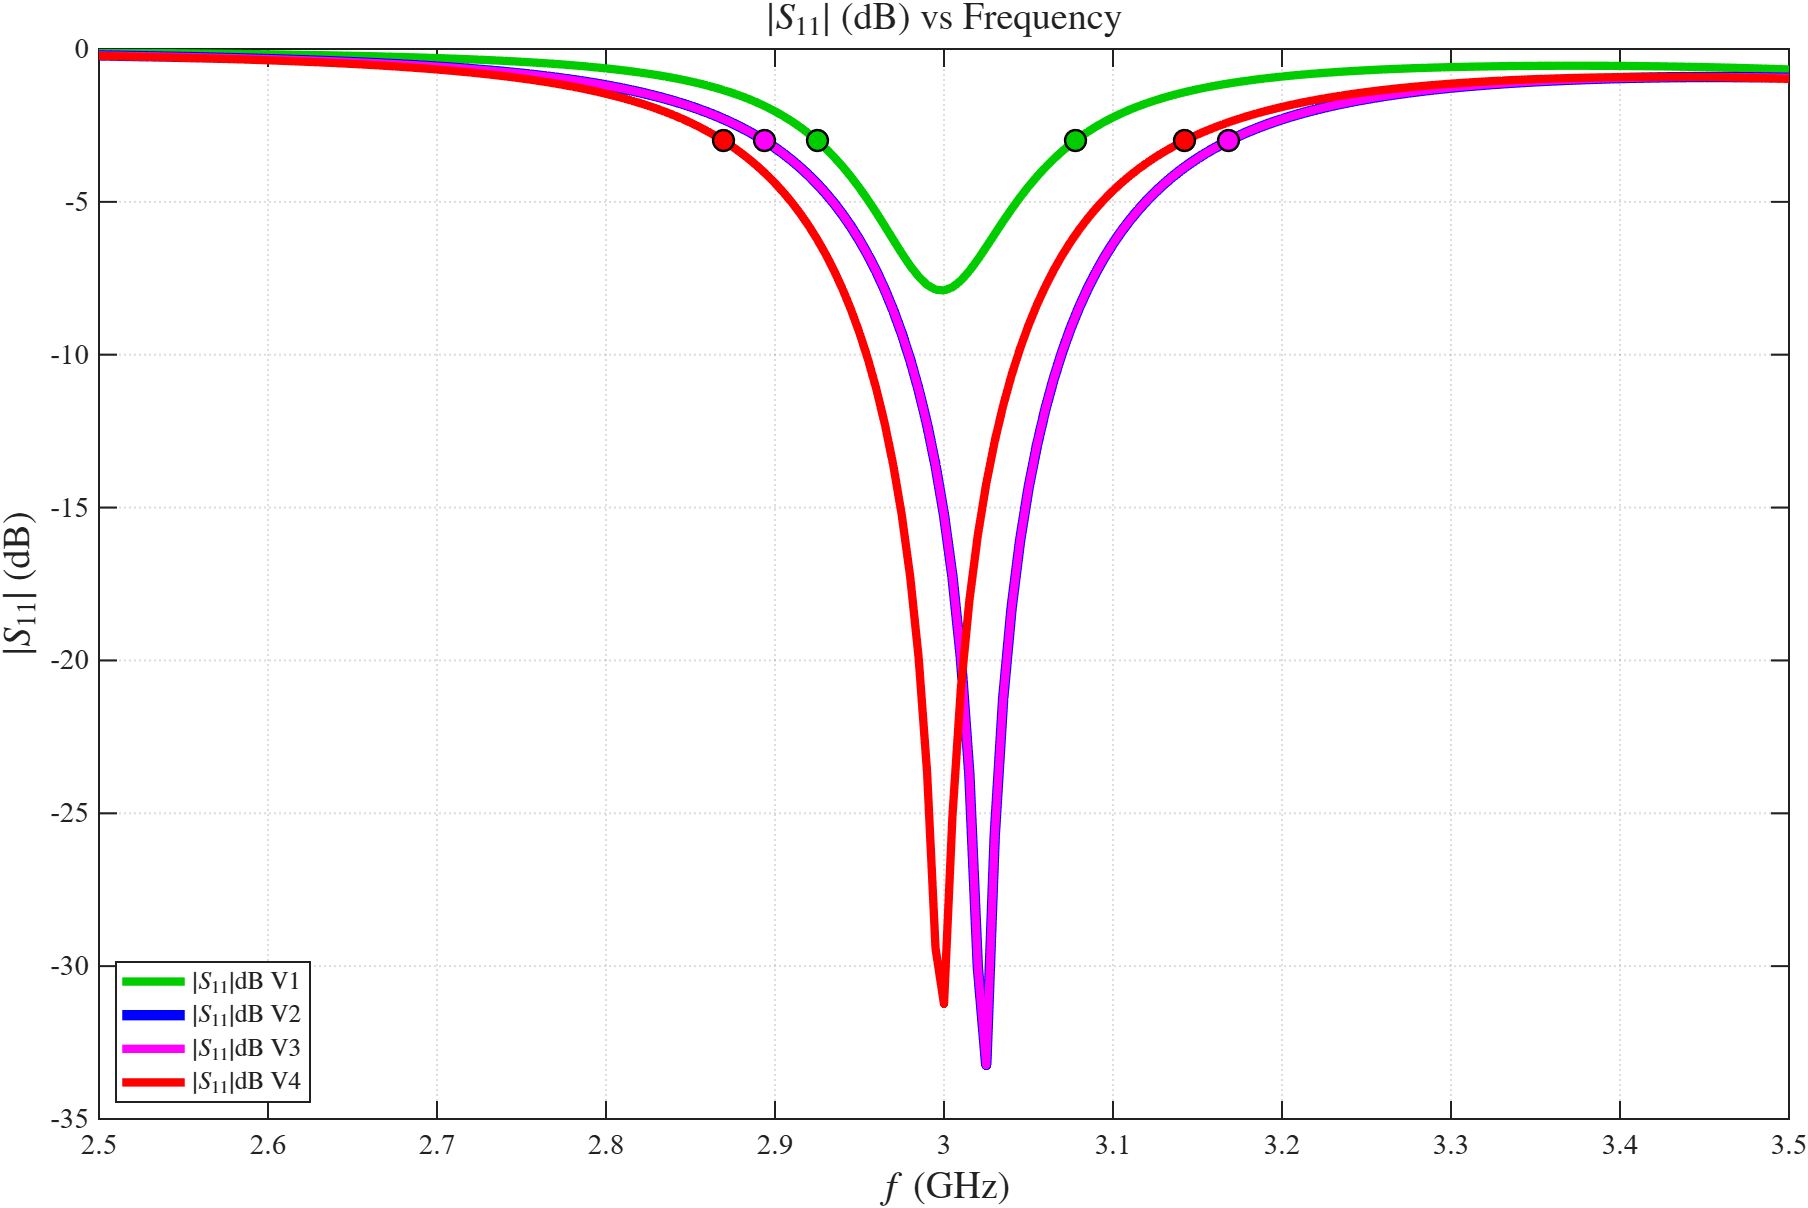
\includegraphics[width=0.95\textwidth,height=0.78\textheight,keepaspectratio,clip,trim=0cm 0.65cm 0cm 0.65cm]{img/Matlab_Figure_1_All_Sweeps_Matlab_3dB.png}
        \caption{$S_{11}$ (dB) vs $f$ (GHz): MATLAB plot of the $-3$~dB points, per optimetric sweep in HFSS.}
    \end{figure}
\end{frame}

%%%%%%%%%%%%%%%%%%%%%%%%%%%%%%%%%%%%%%%%%%%%%%%%%%%%%%%%%%%%%%%%%%%%%%%%%%%%%%%%%%
% APPENDIX IV: REFERENCES
%%%%%%%%%%%%%%%%%%%%%%%%%%%%%%%%%%%%%%%%%%%%%%%%%%%%%%%%%%%%%%%%%%%%%%%%%%%%%%%%%%

\begin{frame}{Appendix IV: References}
    \small
    \textbf{References:}\\
    Ryan Leonard, Aidan Butler, Tommy Nguyen, Fevin Farjado

    \vspace{1em}
    \textbf{Software Tools:}
    \begin{itemize}
        \item Ansys HFSS for electromagnetic simulation
        \item MATLAB for data analysis and visualization
        \item \LaTeX{} for presentation formatting
    \end{itemize}

    \vspace{1em}
    \textbf{Course:}\\
    EE-457/557 Wave Transmission and Reception\\
    Fall 2025
\end{frame}

\end{document}
